\documentclass{l4dc2027}
% If your paper is accepted, please use the "final" option
% for the camera-ready version
% \documentclass[final]{l4dc2027}

% The following packages will be automatically loaded:
% amsmath, amssymb, natbib, graphicx, url, algorithm2e

\usepackage{times}
\usepackage[T1]{fontenc}
\usepackage{booktabs}
\setlength{\emergencystretch}{1.5em} % lets lines with long inline math break instead of running into the margin
% Sub-figures use the \subfigure command of the jmlr class, which clashes with the subfig package.
\graphicspath{{figures/}{experiment-integrator/figures/}{experiment-arm/figures/}{experiment-lightdark/figures/}}

\usepackage{tikz}
\usetikzlibrary{positioning,calc}
\tikzset{
    factor/.style={draw, fill=black, minimum size=3.5mm, inner sep=0pt},
    equality/.style={draw, fill=white, minimum size=3.5mm, inner sep=0pt, font=\scriptsize},
    edgelabel/.style={font=\scriptsize, inner sep=1pt}
}
\usepackage{pgfplots}
\usepackage{circuitikz}
\usepackage{tikz-cd}
% \usetikzlibrary{circuits.ee.IEC}
\usetikzlibrary{intersections}
\usepackage{bm}
\usetikzlibrary{positioning}
\usepgfplotslibrary{fillbetween}
\pgfplotsset{compat=1.5}
\usetikzlibrary{pgfplots.groupplots}
\usetikzlibrary{shapes.geometric,backgrounds}
\newcommand*\circled[2]{\tikz[baseline=(char.base)]{
\node[circle,draw,scale=#2,inner sep=2pt] (char) {#1};}}
\newcommand*\darkcircled[2]{\tikz[baseline=(char.base)]{
\node[circle,draw,scale=#2,inner sep=2pt,fill=darkgrey, text=white] (char) {#1};}}

% \newcommand\esymbol[1]{\tikz[circuit ee IEC] \draw node [#1,anchor=west,name=s] {};}
\ctikzset{bipoles/length=.6cm}
\newcommand\esymbol[1]{\begin{circuitikz}
\draw (0,0) to [#1] (.1,0); \end{circuitikz}}

\usepackage{tikz}
\usepackage{xifthen}

\pgfdeclarelayer{bg}    % declare background layer
\pgfsetlayers{bg,main}  % set the order of the layers (main is the standard layer)
\definecolor{beige}{RGB}{245, 245, 220}

            

\definecolor{darkgrey}{RGB}{75, 75, 75}
\definecolor{lightgrey}{RGB}{250, 250, 250}
% \newcommand*\circled[1]{\tikz[baseline=(char.base)]{            \node[shape=circle,draw,inner sep=1pt] (char) {#1};}}
\newcommand*\smallcircled[1]{\tikz[baseline=(char.base)]{
            \node[shape=circle,draw,inner sep=0pt,minimum width=3.5mm] (char) {#1};}}

\newcommand*\blacksmallcircled[1]{\tikz[baseline=(char.base)]{
            \node[shape=circle,fill=darkgrey, text=white, draw,inner sep=0pt,minimum width=3.5mm] (char) {#1};}}
            
\newcommand*\redsmallcircled[1]{\tikz[baseline=(char.base)]{
            \node[shape=circle, draw=red, text=red,draw,inner sep=0pt,minimum width=3.5mm] (char) {#1};}}
            
\newcommand*\reddarksmallcircled[1]{\tikz[baseline=(char.base)]{
           \node[shape=circle, draw=red, text=white,,fill=red, draw,inner sep=0pt,minimum width=3.5mm] (char) {#1};}}




\usetikzlibrary{calc, arrows, fit, positioning, patterns, decorations.pathreplacing, shapes}
\tikzstyle{dash} = [dashed, -latex,>=latex]
\tikzstyle{line} = [draw, -latex,>=latex]
\tikzstyle{smallbox} = [draw, minimum size=5.0mm]
\tikzstyle{box} = [draw, minimum size=7.0mm]
\tikzstyle{bigbox} = [draw, minimum size=10.0mm]
\tikzstyle{rectangle} = [draw, minimum width=10.0mm, minimum height=20.0mm]
\tikzstyle{switch} = [trapezium, trapezium angle=120, draw, rotate=90,  inner ysep=5pt, outer sep=5pt,
minimum height=7mm, minimum width=7mm]
\tikzstyle{roundbox} = [draw, circle, inner sep=0pt, minimum size=3mm]
\tikzstyle{clamped} = [draw, fill=darkgrey, minimum size=0.15cm]
\tikzstyle{msgcircle} = [shape=circle, draw, inner sep=0pt, minimum size=4mm, fill=white, font=\scriptsize]
\tikzstyle{darkmsgcircle} = [shape=circle, draw, inner sep=0pt, minimum size=4mm, fill=darkgrey, text=white, font=\scriptsize]
\tikzstyle{redmsgcircle} = [shape=circle, draw=red, inner sep=0pt, minimum size=4mm, text=red, font=\scriptsize]
\tikzstyle{reddarkmsgcircle} = [shape=circle, draw=red, inner sep=0pt, minimum size=4mm, fill=red, text=white, font=\scriptsize]
\tikzstyle{msgdoublecircle} = [shape=circle, double, double distance=1.5pt, draw, inner sep=0pt, minimum size=5mm, fill=white]
\tikzstyle{darkmsgdoublecircle} = [shape=circle, double, double distance=1.5pt, draw, inner sep=0pt, minimum size=5mm, fill=darkgrey, text=white, font=\bfseries]
% \tikzstyle{rectangle} = [shape=rectangle, draw, minimum size=20mm]

% \draw (0,0) rectangle (4,4);
% Plate notation argument order: x-left, x-right, y-top, y-bottom
\newcommand{\brackets}[4]{
      \draw[dotted, rounded corners=0.3cm, line width = 1pt] ($({#1},{#3})+(-0.3,0)$) -- ($({#1},{#3})+(-0.3,0.3)$) -- ($({#2},{#3})+(0.3,0.3)$) -- ($({#2},{#3})+(0.3,0)$);
      \draw[dotted, rounded corners=0.3cm, line width = 1pt] ($({#1},{#4})+(-0.3,0)$) -- ($({#1},{#4})+(-0.3,-0.3)$) -- ($({#2},{#4})+(0.3,-0.3)$) -- ($({#2},{#4})+(0.3,0)$);}

% Message notation argument order:
%     Circle position relative to arrow [up, down, left, right];
%     Arrow direction [up, down, left, right];
%     Start node coordinate;
%     End node coordinate
%     Position along edge;
%     Message text;
\newcommand{\msg}[6]{
      % Circle left arrow down
      \ifthenelse{\isin{#1}{left} \AND \isin{#2}{down}}{
            \coordinate (anchor) at ($({#3})!{#5}!({#4})$);
            \node[xshift=-6.0mm] at (anchor) {#6};
            \node[xshift=-1.0mm] at (anchor) {$\downarrow$};
      }{}
      % Circle right arrow down
      \ifthenelse{\isin{#1}{right} \AND \isin{#2}{down}}{
            \coordinate (anchor) at ($({#3})!{#5}!({#4})$);
            \node[xshift=6.0mm] at (anchor) {#6};
            \node[xshift=1.0mm] at (anchor) {$\downarrow$};
      }{}

      % Circle down arrow right
      \ifthenelse{\isin{#1}{down} \AND \isin{#2}{right}}{
            \coordinate (anchor) at ($({#3})!{#5}!({#4})$);
            \node[ yshift=-4.0mm] at (anchor) {#6};
            \node[yshift=-1.0mm] at (anchor) {$\rightarrow$};
      }{}
      % Circle up arrow right
      \ifthenelse{\isin{#1}{up} \AND \isin{#2}{right}}{
            \coordinate (anchor) at ($({#3})!{#5}!({#4})$);
            \node[ yshift=4.0mm] at (anchor) {#6};
            \node[yshift=1.0mm] at (anchor) {$\rightarrow$};
      }{}

      % Circle down arrow left
      \ifthenelse{\isin{#1}{down} \AND \isin{#2}{left}}{
            \coordinate (anchor) at ($({#3})!{#5}!({#4})$);
            \node[ yshift=-4.0mm] at (anchor) {#6};
            \node[yshift=-1.0mm] at (anchor) {$\leftarrow$};
      }{}
      % Circle up arrow left
      \ifthenelse{\isin{#1}{up} \AND \isin{#2}{left}}{
            \coordinate (anchor) at ($({#3})!{#5}!({#4})$);
            \node[ yshift=4.0mm] at (anchor) {#6};
            \node[yshift=1.0mm] at (anchor) {$\leftarrow$};
      }{}

      % Circle left arrow down
      \ifthenelse{\isin{#1}{left} \AND \isin{#2}{up}}{
            \coordinate (anchor) at ($({#3})!{#5}!({#4})$);
            \node[ xshift=-6.0mm] at (anchor) {#6};
            \node[xshift=-1.0mm] at (anchor) {$\uparrow$};
      }{}
      % Circle right arrow down
      \ifthenelse{\isin{#1}{right} \AND \isin{#2}{up}}{
            \coordinate (anchor) at ($({#3})!{#5}!({#4})$);
            \node[ xshift=6.0mm] at (anchor) {#6};
            \node[xshift=1.0mm] at (anchor) {$\uparrow$};
      }{}
}

\newcommand{\msgcircle}[6]{
      % Circle left arrow down
      \ifthenelse{\isin{#1}{left} \AND \isin{#2}{down}}{
            \coordinate (anchor) at ($({#3})!{#5}!({#4})$);
            \node[msgcircle,xshift=-5.0mm] at (anchor) {#6};
            \node[xshift=-1.5mm] at (anchor) {$\downarrow$};
      }{}
      % Circle right arrow down
      \ifthenelse{\isin{#1}{right} \AND \isin{#2}{down}}{
            \coordinate (anchor) at ($({#3})!{#5}!({#4})$);
            \node[msgcircle,xshift=5.0mm] at (anchor) {#6};
            \node[xshift=1.5mm] at (anchor) {$\downarrow$};
      }{}

      % Circle down arrow right
      \ifthenelse{\isin{#1}{down} \AND \isin{#2}{right}}{
            \coordinate (anchor) at ($({#3})!{#5}!({#4})$);
            \node[msgcircle, yshift=-5.0mm] at (anchor) {#6};
            \node[yshift=-2.0mm] at (anchor) {$\rightarrow$};
      }{}
      % Circle up arrow right
      \ifthenelse{\isin{#1}{up} \AND \isin{#2}{right}}{
            \coordinate (anchor) at ($({#3})!{#5}!({#4})$);
            \node[msgcircle, yshift=5.0mm] at (anchor) {#6};
            \node[yshift=2.0mm] at (anchor) {$\rightarrow$};
      }{}

      % Circle down arrow left
      \ifthenelse{\isin{#1}{down} \AND \isin{#2}{left}}{
            \coordinate (anchor) at ($({#3})!{#5}!({#4})$);
            \node[msgcircle, yshift=-5.0mm] at (anchor) {#6};
            \node[yshift=-2.0mm] at (anchor) {$\leftarrow$};
      }{}
      % Circle up arrow left
      \ifthenelse{\isin{#1}{up} \AND \isin{#2}{left}}{
            \coordinate (anchor) at ($({#3})!{#5}!({#4})$);
            \node[msgcircle, yshift=5.0mm] at (anchor) {#6};
            \node[yshift=2.0mm] at (anchor) {$\leftarrow$};
      }{}

      % Circle left arrow down
      \ifthenelse{\isin{#1}{left} \AND \isin{#2}{up}}{
            \coordinate (anchor) at ($({#3})!{#5}!({#4})$);
            \node[msgcircle, xshift=-5.0mm] at (anchor) {#6};
            \node[xshift=-1.5mm] at (anchor) {$\uparrow$};
      }{}
      % Circle right arrow down
      \ifthenelse{\isin{#1}{right} \AND \isin{#2}{up}}{
            \coordinate (anchor) at ($({#3})!{#5}!({#4})$);
            \node[msgcircle, xshift=5.0mm] at (anchor) {#6};
            \node[xshift=1.5mm] at (anchor) {$\uparrow$};
      }{}
}

\newcommand{\darkmsg}[6]{
      % Circle left arrow down
      \ifthenelse{\isin{#1}{left} \AND \isin{#2}{down}}{
            \coordinate (anchor) at ($({#3})!{#5}!({#4})$);
            \node[darkmsgcircle, xshift=-5mm] at (anchor) {#6};
            \node[xshift=-1.5mm] at (anchor) {$\downarrow$};
      }{}
      % Circle right arrow down
      \ifthenelse{\isin{#1}{right} \AND \isin{#2}{down}}{
            \coordinate (anchor) at ($({#3})!{#5}!({#4})$);
            \node[darkmsgcircle, xshift=5mm] at (anchor) {#6};
            \node[xshift=1.5mm] at (anchor) {$\downarrow$};
      }{}

      % Circle down arrow right
      \ifthenelse{\isin{#1}{down} \AND \isin{#2}{right}}{
            \coordinate (anchor) at ($({#3})!{#5}!({#4})$);
            \node[darkmsgcircle, yshift=-5.0mm] at (anchor) {#6};
            \node[yshift=-2.0mm] at (anchor) {$\rightarrow$};
      }{}
      % Circle up arrow right
      \ifthenelse{\isin{#1}{up} \AND \isin{#2}{right}}{
            \coordinate (anchor) at ($({#3})!{#5}!({#4})$);
            \node[darkmsgcircle, yshift=5.0mm] at (anchor) {#6};
            \node[yshift=2.0mm] at (anchor) {$\rightarrow$};
      }{}

      % Circle down arrow left
      \ifthenelse{\isin{#1}{down} \AND \isin{#2}{left}}{
            \coordinate (anchor) at ($({#3})!{#5}!({#4})$);
            \node[darkmsgcircle, yshift=-5.0mm] at (anchor) {#6};
            \node[yshift=-2.0mm] at (anchor) {$\leftarrow$};
      }{}
      % Circle up arrow left
      \ifthenelse{\isin{#1}{up} \AND \isin{#2}{left}}{
            \coordinate (anchor) at ($({#3})!{#5}!({#4})$);
            \node[darkmsgcircle, yshift=5.0mm] at (anchor) {#6};
            \node[yshift=2.0mm] at (anchor) {$\leftarrow$};
      }{}

      % Circle left arrow down
      \ifthenelse{\isin{#1}{left} \AND \isin{#2}{up}}{
            \coordinate (anchor) at ($({#3})!{#5}!({#4})$);
            \node[darkmsgcircle, xshift=-5.0mm] at (anchor) {#6};
            \node[xshift=-1.5mm] at (anchor) {$\uparrow$};
      }{}
      % Circle right arrow down
      \ifthenelse{\isin{#1}{right} \AND \isin{#2}{up}}{
            \coordinate (anchor) at ($({#3})!{#5}!({#4})$);
            \node[darkmsgcircle, xshift=5.0mm] at (anchor) {#6};
            \node[xshift=1.5mm] at (anchor) {$\uparrow$};
      }{}
}

\newcommand{\redbackmsg}[6]{
      % Circle left arrow down
      \ifthenelse{\isin{#1}{left} \AND \isin{#2}{down}}{
            \coordinate (anchor) at ($({#3})!{#5}!({#4})$);
            \node[reddarkmsgcircle, xshift=-5mm] at (anchor) {#6};
            \node[xshift=-1.5mm] at (anchor) {$\downarrow$};
      }{}
      % Circle right arrow down
      \ifthenelse{\isin{#1}{right} \AND \isin{#2}{down}}{
            \coordinate (anchor) at ($({#3})!{#5}!({#4})$);
            \node[reddarkmsgcircle, xshift=5mm] at (anchor) {#6};
            \node[xshift=1.5mm] at (anchor) {$\downarrow$};
      }{}

      % Circle down arrow right
      \ifthenelse{\isin{#1}{down} \AND \isin{#2}{right}}{
            \coordinate (anchor) at ($({#3})!{#5}!({#4})$);
            \node[reddarkmsgcircle, yshift=-5.0mm] at (anchor) {#6};
            \node[yshift=-2.0mm] at (anchor) {$\rightarrow$};
      }{}
      % Circle up arrow right
      \ifthenelse{\isin{#1}{up} \AND \isin{#2}{right}}{
            \coordinate (anchor) at ($({#3})!{#5}!({#4})$);
            \node[reddarkmsgcircle, yshift=5.0mm] at (anchor) {#6};
            \node[yshift=2.0mm] at (anchor) {$\rightarrow$};
      }{}

      % Circle down arrow left
      \ifthenelse{\isin{#1}{down} \AND \isin{#2}{left}}{
            \coordinate (anchor) at ($({#3})!{#5}!({#4})$);
            \node[reddarkmsgcircle, yshift=-5.0mm] at (anchor) {#6};
            \node[yshift=-2.0mm] at (anchor) {$\leftarrow$};
      }{}
      % Circle up arrow left
      \ifthenelse{\isin{#1}{up} \AND \isin{#2}{left}}{
            \coordinate (anchor) at ($({#3})!{#5}!({#4})$);
            \node[reddarkmsgcircle, yshift=5.0mm] at (anchor) {#6};
            \node[yshift=2.0mm] at (anchor) {$\leftarrow$};
      }{}

      % Circle left arrow down
      \ifthenelse{\isin{#1}{left} \AND \isin{#2}{up}}{
            \coordinate (anchor) at ($({#3})!{#5}!({#4})$);
            \node[reddarkmsgcircle, xshift=-5.0mm] at (anchor) {#6};
            \node[xshift=-1.5mm] at (anchor) {$\uparrow$};
      }{}
      % Circle right arrow down
      \ifthenelse{\isin{#1}{right} \AND \isin{#2}{up}}{
            \coordinate (anchor) at ($({#3})!{#5}!({#4})$);
            \node[reddarkmsgcircle, xshift=5.0mm] at (anchor) {#6};
            \node[xshift=1.5mm] at (anchor) {$\uparrow$};
      }{}
}

\newcommand{\redmsg}[6]{
      % Circle left arrow down
      \ifthenelse{\isin{#1}{left} \AND \isin{#2}{down}}{
            \coordinate (anchor) at ($({#3})!{#5}!({#4})$);
            \node[redmsgcircle, xshift=-5mm] at (anchor) {#6};
            \node[xshift=-1.5mm] at (anchor) {$\downarrow$};
      }{}
      % Circle right arrow down
      \ifthenelse{\isin{#1}{right} \AND \isin{#2}{down}}{
            \coordinate (anchor) at ($({#3})!{#5}!({#4})$);
            \node[redmsgcircle, xshift=5mm] at (anchor) {#6};
            \node[xshift=1.5mm] at (anchor) {$\downarrow$};
      }{}

      % Circle down arrow right
      \ifthenelse{\isin{#1}{down} \AND \isin{#2}{right}}{
            \coordinate (anchor) at ($({#3})!{#5}!({#4})$);
            \node[redmsgcircle, yshift=-5.0mm] at (anchor) {#6};
            \node[yshift=-2.0mm] at (anchor) {$\rightarrow$};
      }{}
      % Circle up arrow right
      \ifthenelse{\isin{#1}{up} \AND \isin{#2}{right}}{
            \coordinate (anchor) at ($({#3})!{#5}!({#4})$);
            \node[redmsgcircle, yshift=5.0mm] at (anchor) {#6};
            \node[yshift=2.0mm] at (anchor) {$\rightarrow$};
      }{}

      % Circle down arrow left
      \ifthenelse{\isin{#1}{down} \AND \isin{#2}{left}}{
            \coordinate (anchor) at ($({#3})!{#5}!({#4})$);
            \node[redmsgcircle, yshift=-5.0mm] at (anchor) {#6};
            \node[yshift=-2.0mm] at (anchor) {$\leftarrow$};
      }{}
      % Circle up arrow left
      \ifthenelse{\isin{#1}{up} \AND \isin{#2}{left}}{
            \coordinate (anchor) at ($({#3})!{#5}!({#4})$);
            \node[redmsgcircle, yshift=5.0mm] at (anchor) {#6};
            \node[yshift=2.0mm] at (anchor) {$\leftarrow$};
      }{}

      % Circle left arrow down
      \ifthenelse{\isin{#1}{left} \AND \isin{#2}{up}}{
            \coordinate (anchor) at ($({#3})!{#5}!({#4})$);
            \node[redmsgcircle, xshift=-5.0mm] at (anchor) {#6};
            \node[xshift=-1.5mm] at (anchor) {$\uparrow$};
      }{}
      % Circle right arrow down
      \ifthenelse{\isin{#1}{right} \AND \isin{#2}{up}}{
            \coordinate (anchor) at ($({#3})!{#5}!({#4})$);
            \node[redmsgcircle, xshift=5.0mm] at (anchor) {#6};
            \node[xshift=1.5mm] at (anchor) {$\uparrow$};
      }{}
}

\newcommand{\bwmsg}[6]{
      % doublecircle left arrow down
      \ifthenelse{\isin{#1}{left} \AND \isin{#2}{down}}{
            \coordinate (anchor) at ($({#3})!{#5}!({#4})$);
            \node[msgdoublecircle, xshift=-5.5mm] at (anchor) {#6};
            \node[xshift=-1.5mm] at (anchor) {$\downarrow$};
      }{}
      % doublecircle right arrow down
      \ifthenelse{\isin{#1}{right} \AND \isin{#2}{down}}{
            \coordinate (anchor) at ($({#3})!{#5}!({#4})$);
            \node[msgdoublecircle, xshift=5.5mm] at (anchor) {#6};
            \node[xshift=1.5mm] at (anchor) {$\downarrow$};
      }{}

      % doublecircle down arrow right
      \ifthenelse{\isin{#1}{down} \AND \isin{#2}{right}}{
            \coordinate (anchor) at ($({#3})!{#5}!({#4})$);
            \node[msgdoublecircle, yshift=-6.0mm] at (anchor) {#6};
            \node[yshift=-2.0mm] at (anchor) {$\rightarrow$};
      }{}
      % doublecircle up arrow right
      \ifthenelse{\isin{#1}{up} \AND \isin{#2}{right}}{
            \coordinate (anchor) at ($({#3})!{#5}!({#4})$);
            \node[msgdoublecircle, yshift=6.0mm] at (anchor) {#6};
            \node[yshift=2.0mm] at (anchor) {$\rightarrow$};
      }{}

      % doublecircle down arrow left
      \ifthenelse{\isin{#1}{down} \AND \isin{#2}{left}}{
            \coordinate (anchor) at ($({#3})!{#5}!({#4})$);
            \node[msgdoublecircle, yshift=-6.0mm] at (anchor) {#6};
            \node[yshift=-2.0mm] at (anchor) {$\leftarrow$};
      }{}
      % doublecircle up arrow left
      \ifthenelse{\isin{#1}{up} \AND \isin{#2}{left}}{
            \coordinate (anchor) at ($({#3})!{#5}!({#4})$);
            \node[msgdoublecircle, yshift=6.0mm] at (anchor) {#6};
            \node[yshift=2.0mm] at (anchor) {$\leftarrow$};
      }{}

      % doublecircle left arrow down
      \ifthenelse{\isin{#1}{left} \AND \isin{#2}{up}}{
            \coordinate (anchor) at ($({#3})!{#5}!({#4})$);
            \node[msgdoublecircle, xshift=-5.5mm] at (anchor) {#6};
            \node[xshift=-1.5mm] at (anchor) {$\uparrow$};
      }{}
      % doublecircle right arrow down
      \ifthenelse{\isin{#1}{right} \AND \isin{#2}{up}}{
            \coordinate (anchor) at ($({#3})!{#5}!({#4})$);
            \node[msgdoublecircle, xshift=5.5mm] at (anchor) {#6};
            \node[xshift=1.5mm] at (anchor) {$\uparrow$};
      }{}
}

% Dark messages
\newcommand{\bwdarkmsg}[6]{
      % doublecircle left arrow down
      \ifthenelse{\isin{#1}{left} \AND \isin{#2}{down}}{
            \coordinate (anchor) at ($({#3})!{#5}!({#4})$);
            \node[darkmsgdoublecircle, xshift=-5.5mm] at (anchor) {#6};
            \node[xshift=-1.5mm] at (anchor) {$\downarrow$};
      }{}
      % doublecircle right arrow down
      \ifthenelse{\isin{#1}{right} \AND \isin{#2}{down}}{
            \coordinate (anchor) at ($({#3})!{#5}!({#4})$);
            \node[darkmsgdoublecircle, xshift=5.5mm] at (anchor) {#6};
            \node[xshift=1.5mm] at (anchor) {$\downarrow$};
      }{}

      % doublecircle down arrow right
      \ifthenelse{\isin{#1}{down} \AND \isin{#2}{right}}{
            \coordinate (anchor) at ($({#3})!{#5}!({#4})$);
            \node[darkmsgdoublecircle, yshift=-6.0mm] at (anchor) {#6};
            \node[yshift=-2.0mm] at (anchor) {$\rightarrow$};
      }{}
      % doublecircle up arrow right
      \ifthenelse{\isin{#1}{up} \AND \isin{#2}{right}}{
            \coordinate (anchor) at ($({#3})!{#5}!({#4})$);
            \node[darkmsgdoublecircle, yshift=6.0mm] at (anchor) {#6};
            \node[yshift=2.0mm] at (anchor) {$\rightarrow$};
      }{}

      % doublecircle down arrow left
      \ifthenelse{\isin{#1}{down} \AND \isin{#2}{left}}{
            \coordinate (anchor) at ($({#3})!{#5}!({#4})$);
            \node[darkmsgdoublecircle, yshift=-6.0mm] at (anchor) {#6};
            \node[yshift=-2.0mm] at (anchor) {$\leftarrow$};
      }{}
      % doublecircle up arrow left
      \ifthenelse{\isin{#1}{up} \AND \isin{#2}{left}}{
            \coordinate (anchor) at ($({#3})!{#5}!({#4})$);
            \node[darkmsgdoublecircle, yshift=6.0mm] at (anchor) {#6};
            \node[yshift=2.0mm] at (anchor) {$\leftarrow$};
      }{}

      % doublecircle left arrow down
      \ifthenelse{\isin{#1}{left} \AND \isin{#2}{up}}{
            \coordinate (anchor) at ($({#3})!{#5}!({#4})$);
            \node[darkmsgdoublecircle, xshift=-5.5mm] at (anchor) {#6};
            \node[xshift=-1.5mm] at (anchor) {$\uparrow$};
      }{}
      % doublecircle right arrow down
      \ifthenelse{\isin{#1}{right} \AND \isin{#2}{up}}{
            \coordinate (anchor) at ($({#3})!{#5}!({#4})$);
            \node[darkmsgdoublecircle, xshift=5.5mm] at (anchor) {#6};
            \node[xshift=1.5mm] at (anchor) {$\uparrow$};
      }{}
}

% nodes style 
\tikzset{mainstyle/.style={fill=white, draw=black, shape=rectangle, align=center}}

\tikzset{dstyle/.style={mainstyle, minimum size=4mm, inner sep=0pt, text width=4mm}}

\tikzset{sstyle/.style={mainstyle, minimum size=5mm, inner sep=0pt, text width=5mm}}

\tikzset{ostyle/.style={fill=darkgrey, draw=black, shape=rectangle, minimum size=0.2cm, inner sep=0pt, text width=2mm}}

% main nodes
\tikzstyle{observation}=[ostyle]
\tikzstyle{deterministic}=[dstyle]
\tikzstyle{stochastic}=[sstyle]

% auxiliary nodes
\tikzstyle{filter}=[mainstyle, minimum width=1cm, minimum height=0.5cm]
\tikzstyle{selector}=[fill=white, draw=black, shape=trapezium, rotate=180, minimum width=1cm, minimum height=0.5cm]

% \newcommand*\circled[1]{\tikz[baseline=(char.base)]{
%             \node[shape=circle,draw,minimum size=4mm,inner sep=0pt] (char) {#1};}}
% \newcommand*\squared[1]{\tikz[baseline=(char.base)]{
%             \node[shape=rectangle,draw,minimum size=5mm,inner sep=0pt] (char) {#1};}}
% Line weight of all graphs: edges, node borders, dashed boxes and message
% circles are drawn semithick (0.6 pt) instead of TikZ's default thin (0.4 pt).
\tikzset{every picture/.append style={semithick}}


% \usepackage{pgfplots}
\usepackage{circuitikz}
\usepackage{tikz-cd}
% \usetikzlibrary{circuits.ee.IEC}
\usetikzlibrary{intersections}
\usepackage{bm}
\usetikzlibrary{positioning}
\usepgfplotslibrary{fillbetween}
\pgfplotsset{compat=1.5}
\usetikzlibrary{pgfplots.groupplots}
\usetikzlibrary{shapes.geometric,backgrounds}
\newcommand*\circled[2]{\tikz[baseline=(char.base)]{
\node[circle,draw,scale=#2,inner sep=2pt] (char) {#1};}}
\newcommand*\darkcircled[2]{\tikz[baseline=(char.base)]{
\node[circle,draw,scale=#2,inner sep=2pt,fill=darkgrey, text=white] (char) {#1};}}

% \newcommand\esymbol[1]{\tikz[circuit ee IEC] \draw node [#1,anchor=west,name=s] {};}
\ctikzset{bipoles/length=.6cm}
\newcommand\esymbol[1]{\begin{circuitikz}
\draw (0,0) to [#1] (.1,0); \end{circuitikz}}

\usepackage{tikz}
\usepackage{xifthen}

\pgfdeclarelayer{bg}    % declare background layer
\pgfsetlayers{bg,main}  % set the order of the layers (main is the standard layer)
\definecolor{beige}{RGB}{245, 245, 220}

            

\definecolor{darkgrey}{RGB}{75, 75, 75}
\definecolor{lightgrey}{RGB}{250, 250, 250}
% \newcommand*\circled[1]{\tikz[baseline=(char.base)]{            \node[shape=circle,draw,inner sep=1pt] (char) {#1};}}
\newcommand*\smallcircled[1]{\tikz[baseline=(char.base)]{
            \node[shape=circle,draw,inner sep=0pt,minimum width=3.5mm] (char) {#1};}}

\newcommand*\blacksmallcircled[1]{\tikz[baseline=(char.base)]{
            \node[shape=circle,fill=darkgrey, text=white, draw,inner sep=0pt,minimum width=3.5mm] (char) {#1};}}
            
\newcommand*\redsmallcircled[1]{\tikz[baseline=(char.base)]{
            \node[shape=circle, draw=red, text=red,draw,inner sep=0pt,minimum width=3.5mm] (char) {#1};}}
            
\newcommand*\reddarksmallcircled[1]{\tikz[baseline=(char.base)]{
           \node[shape=circle, draw=red, text=white,,fill=red, draw,inner sep=0pt,minimum width=3.5mm] (char) {#1};}}




\usetikzlibrary{calc, arrows, fit, positioning, patterns, decorations.pathreplacing, shapes}
\tikzstyle{dash} = [dashed, -latex,>=latex]
\tikzstyle{line} = [draw, -latex,>=latex]
\tikzstyle{smallbox} = [draw, minimum size=5.0mm]
\tikzstyle{box} = [draw, minimum size=7.0mm]
\tikzstyle{bigbox} = [draw, minimum size=10.0mm]
\tikzstyle{rectangle} = [draw, minimum width=10.0mm, minimum height=20.0mm]
\tikzstyle{switch} = [trapezium, trapezium angle=120, draw, rotate=90,  inner ysep=5pt, outer sep=5pt,
minimum height=7mm, minimum width=7mm]
\tikzstyle{roundbox} = [draw, circle, inner sep=0pt, minimum size=3mm]
\tikzstyle{clamped} = [draw, fill=darkgrey, minimum size=0.15cm]
\tikzstyle{msgcircle} = [shape=circle, draw, inner sep=0pt, minimum size=4mm, fill=white, font=\scriptsize]
\tikzstyle{darkmsgcircle} = [shape=circle, draw, inner sep=0pt, minimum size=4mm, fill=darkgrey, text=white, font=\scriptsize]
\tikzstyle{redmsgcircle} = [shape=circle, draw=red, inner sep=0pt, minimum size=4mm, text=red, font=\scriptsize]
\tikzstyle{reddarkmsgcircle} = [shape=circle, draw=red, inner sep=0pt, minimum size=4mm, fill=red, text=white, font=\scriptsize]
\tikzstyle{msgdoublecircle} = [shape=circle, double, double distance=1.5pt, draw, inner sep=0pt, minimum size=5mm, fill=white]
\tikzstyle{darkmsgdoublecircle} = [shape=circle, double, double distance=1.5pt, draw, inner sep=0pt, minimum size=5mm, fill=darkgrey, text=white, font=\bfseries]
% \tikzstyle{rectangle} = [shape=rectangle, draw, minimum size=20mm]

% \draw (0,0) rectangle (4,4);
% Plate notation argument order: x-left, x-right, y-top, y-bottom
\newcommand{\brackets}[4]{
      \draw[dotted, rounded corners=0.3cm, line width = 1pt] ($({#1},{#3})+(-0.3,0)$) -- ($({#1},{#3})+(-0.3,0.3)$) -- ($({#2},{#3})+(0.3,0.3)$) -- ($({#2},{#3})+(0.3,0)$);
      \draw[dotted, rounded corners=0.3cm, line width = 1pt] ($({#1},{#4})+(-0.3,0)$) -- ($({#1},{#4})+(-0.3,-0.3)$) -- ($({#2},{#4})+(0.3,-0.3)$) -- ($({#2},{#4})+(0.3,0)$);}

% Message notation argument order:
%     Circle position relative to arrow [up, down, left, right];
%     Arrow direction [up, down, left, right];
%     Start node coordinate;
%     End node coordinate
%     Position along edge;
%     Message text;
\newcommand{\msg}[6]{
      % Circle left arrow down
      \ifthenelse{\isin{#1}{left} \AND \isin{#2}{down}}{
            \coordinate (anchor) at ($({#3})!{#5}!({#4})$);
            \node[xshift=-6.0mm] at (anchor) {#6};
            \node[xshift=-1.0mm] at (anchor) {$\downarrow$};
      }{}
      % Circle right arrow down
      \ifthenelse{\isin{#1}{right} \AND \isin{#2}{down}}{
            \coordinate (anchor) at ($({#3})!{#5}!({#4})$);
            \node[xshift=6.0mm] at (anchor) {#6};
            \node[xshift=1.0mm] at (anchor) {$\downarrow$};
      }{}

      % Circle down arrow right
      \ifthenelse{\isin{#1}{down} \AND \isin{#2}{right}}{
            \coordinate (anchor) at ($({#3})!{#5}!({#4})$);
            \node[ yshift=-4.0mm] at (anchor) {#6};
            \node[yshift=-1.0mm] at (anchor) {$\rightarrow$};
      }{}
      % Circle up arrow right
      \ifthenelse{\isin{#1}{up} \AND \isin{#2}{right}}{
            \coordinate (anchor) at ($({#3})!{#5}!({#4})$);
            \node[ yshift=4.0mm] at (anchor) {#6};
            \node[yshift=1.0mm] at (anchor) {$\rightarrow$};
      }{}

      % Circle down arrow left
      \ifthenelse{\isin{#1}{down} \AND \isin{#2}{left}}{
            \coordinate (anchor) at ($({#3})!{#5}!({#4})$);
            \node[ yshift=-4.0mm] at (anchor) {#6};
            \node[yshift=-1.0mm] at (anchor) {$\leftarrow$};
      }{}
      % Circle up arrow left
      \ifthenelse{\isin{#1}{up} \AND \isin{#2}{left}}{
            \coordinate (anchor) at ($({#3})!{#5}!({#4})$);
            \node[ yshift=4.0mm] at (anchor) {#6};
            \node[yshift=1.0mm] at (anchor) {$\leftarrow$};
      }{}

      % Circle left arrow down
      \ifthenelse{\isin{#1}{left} \AND \isin{#2}{up}}{
            \coordinate (anchor) at ($({#3})!{#5}!({#4})$);
            \node[ xshift=-6.0mm] at (anchor) {#6};
            \node[xshift=-1.0mm] at (anchor) {$\uparrow$};
      }{}
      % Circle right arrow down
      \ifthenelse{\isin{#1}{right} \AND \isin{#2}{up}}{
            \coordinate (anchor) at ($({#3})!{#5}!({#4})$);
            \node[ xshift=6.0mm] at (anchor) {#6};
            \node[xshift=1.0mm] at (anchor) {$\uparrow$};
      }{}
}

\newcommand{\msgcircle}[6]{
      % Circle left arrow down
      \ifthenelse{\isin{#1}{left} \AND \isin{#2}{down}}{
            \coordinate (anchor) at ($({#3})!{#5}!({#4})$);
            \node[msgcircle,xshift=-5.0mm] at (anchor) {#6};
            \node[xshift=-1.5mm] at (anchor) {$\downarrow$};
      }{}
      % Circle right arrow down
      \ifthenelse{\isin{#1}{right} \AND \isin{#2}{down}}{
            \coordinate (anchor) at ($({#3})!{#5}!({#4})$);
            \node[msgcircle,xshift=5.0mm] at (anchor) {#6};
            \node[xshift=1.5mm] at (anchor) {$\downarrow$};
      }{}

      % Circle down arrow right
      \ifthenelse{\isin{#1}{down} \AND \isin{#2}{right}}{
            \coordinate (anchor) at ($({#3})!{#5}!({#4})$);
            \node[msgcircle, yshift=-5.0mm] at (anchor) {#6};
            \node[yshift=-2.0mm] at (anchor) {$\rightarrow$};
      }{}
      % Circle up arrow right
      \ifthenelse{\isin{#1}{up} \AND \isin{#2}{right}}{
            \coordinate (anchor) at ($({#3})!{#5}!({#4})$);
            \node[msgcircle, yshift=5.0mm] at (anchor) {#6};
            \node[yshift=2.0mm] at (anchor) {$\rightarrow$};
      }{}

      % Circle down arrow left
      \ifthenelse{\isin{#1}{down} \AND \isin{#2}{left}}{
            \coordinate (anchor) at ($({#3})!{#5}!({#4})$);
            \node[msgcircle, yshift=-5.0mm] at (anchor) {#6};
            \node[yshift=-2.0mm] at (anchor) {$\leftarrow$};
      }{}
      % Circle up arrow left
      \ifthenelse{\isin{#1}{up} \AND \isin{#2}{left}}{
            \coordinate (anchor) at ($({#3})!{#5}!({#4})$);
            \node[msgcircle, yshift=5.0mm] at (anchor) {#6};
            \node[yshift=2.0mm] at (anchor) {$\leftarrow$};
      }{}

      % Circle left arrow down
      \ifthenelse{\isin{#1}{left} \AND \isin{#2}{up}}{
            \coordinate (anchor) at ($({#3})!{#5}!({#4})$);
            \node[msgcircle, xshift=-5.0mm] at (anchor) {#6};
            \node[xshift=-1.5mm] at (anchor) {$\uparrow$};
      }{}
      % Circle right arrow down
      \ifthenelse{\isin{#1}{right} \AND \isin{#2}{up}}{
            \coordinate (anchor) at ($({#3})!{#5}!({#4})$);
            \node[msgcircle, xshift=5.0mm] at (anchor) {#6};
            \node[xshift=1.5mm] at (anchor) {$\uparrow$};
      }{}
}

\newcommand{\darkmsg}[6]{
      % Circle left arrow down
      \ifthenelse{\isin{#1}{left} \AND \isin{#2}{down}}{
            \coordinate (anchor) at ($({#3})!{#5}!({#4})$);
            \node[darkmsgcircle, xshift=-5mm] at (anchor) {#6};
            \node[xshift=-1.5mm] at (anchor) {$\downarrow$};
      }{}
      % Circle right arrow down
      \ifthenelse{\isin{#1}{right} \AND \isin{#2}{down}}{
            \coordinate (anchor) at ($({#3})!{#5}!({#4})$);
            \node[darkmsgcircle, xshift=5mm] at (anchor) {#6};
            \node[xshift=1.5mm] at (anchor) {$\downarrow$};
      }{}

      % Circle down arrow right
      \ifthenelse{\isin{#1}{down} \AND \isin{#2}{right}}{
            \coordinate (anchor) at ($({#3})!{#5}!({#4})$);
            \node[darkmsgcircle, yshift=-5.0mm] at (anchor) {#6};
            \node[yshift=-2.0mm] at (anchor) {$\rightarrow$};
      }{}
      % Circle up arrow right
      \ifthenelse{\isin{#1}{up} \AND \isin{#2}{right}}{
            \coordinate (anchor) at ($({#3})!{#5}!({#4})$);
            \node[darkmsgcircle, yshift=5.0mm] at (anchor) {#6};
            \node[yshift=2.0mm] at (anchor) {$\rightarrow$};
      }{}

      % Circle down arrow left
      \ifthenelse{\isin{#1}{down} \AND \isin{#2}{left}}{
            \coordinate (anchor) at ($({#3})!{#5}!({#4})$);
            \node[darkmsgcircle, yshift=-5.0mm] at (anchor) {#6};
            \node[yshift=-2.0mm] at (anchor) {$\leftarrow$};
      }{}
      % Circle up arrow left
      \ifthenelse{\isin{#1}{up} \AND \isin{#2}{left}}{
            \coordinate (anchor) at ($({#3})!{#5}!({#4})$);
            \node[darkmsgcircle, yshift=5.0mm] at (anchor) {#6};
            \node[yshift=2.0mm] at (anchor) {$\leftarrow$};
      }{}

      % Circle left arrow down
      \ifthenelse{\isin{#1}{left} \AND \isin{#2}{up}}{
            \coordinate (anchor) at ($({#3})!{#5}!({#4})$);
            \node[darkmsgcircle, xshift=-5.0mm] at (anchor) {#6};
            \node[xshift=-1.5mm] at (anchor) {$\uparrow$};
      }{}
      % Circle right arrow down
      \ifthenelse{\isin{#1}{right} \AND \isin{#2}{up}}{
            \coordinate (anchor) at ($({#3})!{#5}!({#4})$);
            \node[darkmsgcircle, xshift=5.0mm] at (anchor) {#6};
            \node[xshift=1.5mm] at (anchor) {$\uparrow$};
      }{}
}

\newcommand{\redbackmsg}[6]{
      % Circle left arrow down
      \ifthenelse{\isin{#1}{left} \AND \isin{#2}{down}}{
            \coordinate (anchor) at ($({#3})!{#5}!({#4})$);
            \node[reddarkmsgcircle, xshift=-5mm] at (anchor) {#6};
            \node[xshift=-1.5mm] at (anchor) {$\downarrow$};
      }{}
      % Circle right arrow down
      \ifthenelse{\isin{#1}{right} \AND \isin{#2}{down}}{
            \coordinate (anchor) at ($({#3})!{#5}!({#4})$);
            \node[reddarkmsgcircle, xshift=5mm] at (anchor) {#6};
            \node[xshift=1.5mm] at (anchor) {$\downarrow$};
      }{}

      % Circle down arrow right
      \ifthenelse{\isin{#1}{down} \AND \isin{#2}{right}}{
            \coordinate (anchor) at ($({#3})!{#5}!({#4})$);
            \node[reddarkmsgcircle, yshift=-5.0mm] at (anchor) {#6};
            \node[yshift=-2.0mm] at (anchor) {$\rightarrow$};
      }{}
      % Circle up arrow right
      \ifthenelse{\isin{#1}{up} \AND \isin{#2}{right}}{
            \coordinate (anchor) at ($({#3})!{#5}!({#4})$);
            \node[reddarkmsgcircle, yshift=5.0mm] at (anchor) {#6};
            \node[yshift=2.0mm] at (anchor) {$\rightarrow$};
      }{}

      % Circle down arrow left
      \ifthenelse{\isin{#1}{down} \AND \isin{#2}{left}}{
            \coordinate (anchor) at ($({#3})!{#5}!({#4})$);
            \node[reddarkmsgcircle, yshift=-5.0mm] at (anchor) {#6};
            \node[yshift=-2.0mm] at (anchor) {$\leftarrow$};
      }{}
      % Circle up arrow left
      \ifthenelse{\isin{#1}{up} \AND \isin{#2}{left}}{
            \coordinate (anchor) at ($({#3})!{#5}!({#4})$);
            \node[reddarkmsgcircle, yshift=5.0mm] at (anchor) {#6};
            \node[yshift=2.0mm] at (anchor) {$\leftarrow$};
      }{}

      % Circle left arrow down
      \ifthenelse{\isin{#1}{left} \AND \isin{#2}{up}}{
            \coordinate (anchor) at ($({#3})!{#5}!({#4})$);
            \node[reddarkmsgcircle, xshift=-5.0mm] at (anchor) {#6};
            \node[xshift=-1.5mm] at (anchor) {$\uparrow$};
      }{}
      % Circle right arrow down
      \ifthenelse{\isin{#1}{right} \AND \isin{#2}{up}}{
            \coordinate (anchor) at ($({#3})!{#5}!({#4})$);
            \node[reddarkmsgcircle, xshift=5.0mm] at (anchor) {#6};
            \node[xshift=1.5mm] at (anchor) {$\uparrow$};
      }{}
}

\newcommand{\redmsg}[6]{
      % Circle left arrow down
      \ifthenelse{\isin{#1}{left} \AND \isin{#2}{down}}{
            \coordinate (anchor) at ($({#3})!{#5}!({#4})$);
            \node[redmsgcircle, xshift=-5mm] at (anchor) {#6};
            \node[xshift=-1.5mm] at (anchor) {$\downarrow$};
      }{}
      % Circle right arrow down
      \ifthenelse{\isin{#1}{right} \AND \isin{#2}{down}}{
            \coordinate (anchor) at ($({#3})!{#5}!({#4})$);
            \node[redmsgcircle, xshift=5mm] at (anchor) {#6};
            \node[xshift=1.5mm] at (anchor) {$\downarrow$};
      }{}

      % Circle down arrow right
      \ifthenelse{\isin{#1}{down} \AND \isin{#2}{right}}{
            \coordinate (anchor) at ($({#3})!{#5}!({#4})$);
            \node[redmsgcircle, yshift=-5.0mm] at (anchor) {#6};
            \node[yshift=-2.0mm] at (anchor) {$\rightarrow$};
      }{}
      % Circle up arrow right
      \ifthenelse{\isin{#1}{up} \AND \isin{#2}{right}}{
            \coordinate (anchor) at ($({#3})!{#5}!({#4})$);
            \node[redmsgcircle, yshift=5.0mm] at (anchor) {#6};
            \node[yshift=2.0mm] at (anchor) {$\rightarrow$};
      }{}

      % Circle down arrow left
      \ifthenelse{\isin{#1}{down} \AND \isin{#2}{left}}{
            \coordinate (anchor) at ($({#3})!{#5}!({#4})$);
            \node[redmsgcircle, yshift=-5.0mm] at (anchor) {#6};
            \node[yshift=-2.0mm] at (anchor) {$\leftarrow$};
      }{}
      % Circle up arrow left
      \ifthenelse{\isin{#1}{up} \AND \isin{#2}{left}}{
            \coordinate (anchor) at ($({#3})!{#5}!({#4})$);
            \node[redmsgcircle, yshift=5.0mm] at (anchor) {#6};
            \node[yshift=2.0mm] at (anchor) {$\leftarrow$};
      }{}

      % Circle left arrow down
      \ifthenelse{\isin{#1}{left} \AND \isin{#2}{up}}{
            \coordinate (anchor) at ($({#3})!{#5}!({#4})$);
            \node[redmsgcircle, xshift=-5.0mm] at (anchor) {#6};
            \node[xshift=-1.5mm] at (anchor) {$\uparrow$};
      }{}
      % Circle right arrow down
      \ifthenelse{\isin{#1}{right} \AND \isin{#2}{up}}{
            \coordinate (anchor) at ($({#3})!{#5}!({#4})$);
            \node[redmsgcircle, xshift=5.0mm] at (anchor) {#6};
            \node[xshift=1.5mm] at (anchor) {$\uparrow$};
      }{}
}

\newcommand{\bwmsg}[6]{
      % doublecircle left arrow down
      \ifthenelse{\isin{#1}{left} \AND \isin{#2}{down}}{
            \coordinate (anchor) at ($({#3})!{#5}!({#4})$);
            \node[msgdoublecircle, xshift=-5.5mm] at (anchor) {#6};
            \node[xshift=-1.5mm] at (anchor) {$\downarrow$};
      }{}
      % doublecircle right arrow down
      \ifthenelse{\isin{#1}{right} \AND \isin{#2}{down}}{
            \coordinate (anchor) at ($({#3})!{#5}!({#4})$);
            \node[msgdoublecircle, xshift=5.5mm] at (anchor) {#6};
            \node[xshift=1.5mm] at (anchor) {$\downarrow$};
      }{}

      % doublecircle down arrow right
      \ifthenelse{\isin{#1}{down} \AND \isin{#2}{right}}{
            \coordinate (anchor) at ($({#3})!{#5}!({#4})$);
            \node[msgdoublecircle, yshift=-6.0mm] at (anchor) {#6};
            \node[yshift=-2.0mm] at (anchor) {$\rightarrow$};
      }{}
      % doublecircle up arrow right
      \ifthenelse{\isin{#1}{up} \AND \isin{#2}{right}}{
            \coordinate (anchor) at ($({#3})!{#5}!({#4})$);
            \node[msgdoublecircle, yshift=6.0mm] at (anchor) {#6};
            \node[yshift=2.0mm] at (anchor) {$\rightarrow$};
      }{}

      % doublecircle down arrow left
      \ifthenelse{\isin{#1}{down} \AND \isin{#2}{left}}{
            \coordinate (anchor) at ($({#3})!{#5}!({#4})$);
            \node[msgdoublecircle, yshift=-6.0mm] at (anchor) {#6};
            \node[yshift=-2.0mm] at (anchor) {$\leftarrow$};
      }{}
      % doublecircle up arrow left
      \ifthenelse{\isin{#1}{up} \AND \isin{#2}{left}}{
            \coordinate (anchor) at ($({#3})!{#5}!({#4})$);
            \node[msgdoublecircle, yshift=6.0mm] at (anchor) {#6};
            \node[yshift=2.0mm] at (anchor) {$\leftarrow$};
      }{}

      % doublecircle left arrow down
      \ifthenelse{\isin{#1}{left} \AND \isin{#2}{up}}{
            \coordinate (anchor) at ($({#3})!{#5}!({#4})$);
            \node[msgdoublecircle, xshift=-5.5mm] at (anchor) {#6};
            \node[xshift=-1.5mm] at (anchor) {$\uparrow$};
      }{}
      % doublecircle right arrow down
      \ifthenelse{\isin{#1}{right} \AND \isin{#2}{up}}{
            \coordinate (anchor) at ($({#3})!{#5}!({#4})$);
            \node[msgdoublecircle, xshift=5.5mm] at (anchor) {#6};
            \node[xshift=1.5mm] at (anchor) {$\uparrow$};
      }{}
}

% Dark messages
\newcommand{\bwdarkmsg}[6]{
      % doublecircle left arrow down
      \ifthenelse{\isin{#1}{left} \AND \isin{#2}{down}}{
            \coordinate (anchor) at ($({#3})!{#5}!({#4})$);
            \node[darkmsgdoublecircle, xshift=-5.5mm] at (anchor) {#6};
            \node[xshift=-1.5mm] at (anchor) {$\downarrow$};
      }{}
      % doublecircle right arrow down
      \ifthenelse{\isin{#1}{right} \AND \isin{#2}{down}}{
            \coordinate (anchor) at ($({#3})!{#5}!({#4})$);
            \node[darkmsgdoublecircle, xshift=5.5mm] at (anchor) {#6};
            \node[xshift=1.5mm] at (anchor) {$\downarrow$};
      }{}

      % doublecircle down arrow right
      \ifthenelse{\isin{#1}{down} \AND \isin{#2}{right}}{
            \coordinate (anchor) at ($({#3})!{#5}!({#4})$);
            \node[darkmsgdoublecircle, yshift=-6.0mm] at (anchor) {#6};
            \node[yshift=-2.0mm] at (anchor) {$\rightarrow$};
      }{}
      % doublecircle up arrow right
      \ifthenelse{\isin{#1}{up} \AND \isin{#2}{right}}{
            \coordinate (anchor) at ($({#3})!{#5}!({#4})$);
            \node[darkmsgdoublecircle, yshift=6.0mm] at (anchor) {#6};
            \node[yshift=2.0mm] at (anchor) {$\rightarrow$};
      }{}

      % doublecircle down arrow left
      \ifthenelse{\isin{#1}{down} \AND \isin{#2}{left}}{
            \coordinate (anchor) at ($({#3})!{#5}!({#4})$);
            \node[darkmsgdoublecircle, yshift=-6.0mm] at (anchor) {#6};
            \node[yshift=-2.0mm] at (anchor) {$\leftarrow$};
      }{}
      % doublecircle up arrow left
      \ifthenelse{\isin{#1}{up} \AND \isin{#2}{left}}{
            \coordinate (anchor) at ($({#3})!{#5}!({#4})$);
            \node[darkmsgdoublecircle, yshift=6.0mm] at (anchor) {#6};
            \node[yshift=2.0mm] at (anchor) {$\leftarrow$};
      }{}

      % doublecircle left arrow down
      \ifthenelse{\isin{#1}{left} \AND \isin{#2}{up}}{
            \coordinate (anchor) at ($({#3})!{#5}!({#4})$);
            \node[darkmsgdoublecircle, xshift=-5.5mm] at (anchor) {#6};
            \node[xshift=-1.5mm] at (anchor) {$\uparrow$};
      }{}
      % doublecircle right arrow down
      \ifthenelse{\isin{#1}{right} \AND \isin{#2}{up}}{
            \coordinate (anchor) at ($({#3})!{#5}!({#4})$);
            \node[darkmsgdoublecircle, xshift=5.5mm] at (anchor) {#6};
            \node[xshift=1.5mm] at (anchor) {$\uparrow$};
      }{}
}

% nodes style 
\tikzset{mainstyle/.style={fill=white, draw=black, shape=rectangle, align=center}}

\tikzset{dstyle/.style={mainstyle, minimum size=4mm, inner sep=0pt, text width=4mm}}

\tikzset{sstyle/.style={mainstyle, minimum size=5mm, inner sep=0pt, text width=5mm}}

\tikzset{ostyle/.style={fill=darkgrey, draw=black, shape=rectangle, minimum size=0.2cm, inner sep=0pt, text width=2mm}}

% main nodes
\tikzstyle{observation}=[ostyle]
\tikzstyle{deterministic}=[dstyle]
\tikzstyle{stochastic}=[sstyle]

% auxiliary nodes
\tikzstyle{filter}=[mainstyle, minimum width=1cm, minimum height=0.5cm]
\tikzstyle{selector}=[fill=white, draw=black, shape=trapezium, rotate=180, minimum width=1cm, minimum height=0.5cm]

% \newcommand*\circled[1]{\tikz[baseline=(char.base)]{
%             \node[shape=circle,draw,minimum size=4mm,inner sep=0pt] (char) {#1};}}
% \newcommand*\squared[1]{\tikz[baseline=(char.base)]{
%             \node[shape=rectangle,draw,minimum size=5mm,inner sep=0pt] (char) {#1};}}
% Line weight of all graphs: edges, node borders, dashed boxes and message
% circles are drawn semithick (0.6 pt) instead of TikZ's default thin (0.4 pt).
\tikzset{every picture/.append style={semithick}}

\newcommand*\wcircled[1]{\tikz[baseline=(char.base)]{\node[shape=circle,draw,minimum size=4mm,inner sep=0pt] (char) {#1};}}

\usepackage[]{todonotes}
% \usepackage[disable]{todonotes}
\newcommand{\wmk}[2][] {\todo[inline,backgroundcolor=green!20!white, #1]{(Wouter) #2}}
\newcommand{\claude}[2][] {\todo[inline,backgroundcolor=red!20!white, #1]{(Claude) #2}}

\newcommand{\bfy}{\mathbf{y}}
\newcommand{\bfx}{\mathbf{x}}
\newcommand{\bfz}{\mathbf{z}}
\newcommand{\bfu}{\mathbf{u}}
\def\rmd{\mathrm{d}}
\def\cN{\mathcal{N}}
\def\cF{\mathcal{F}}
\def\cG{\mathcal{G}}
\def\cJ{\mathcal{J}}
\def\cD{\mathcal{D}}
\def\cU{\mathcal{U}}
\def\-{\text{-}}
\def\+{\text{+}}
\def\tm{\! - \!}
\def\tp{\! + \!}
\def\tr{\text{tr}}
\newcommand\given[1][]{\,#1\vert\,}
\newcommand{\E}{\mathbb{E}}
\newcommand{\KL}{D_{\mathrm{KL}}}
\newcommand{\mup}{\nu^{\uparrow}}
\newcommand{\mback}{\overleftarrow{\nu}}
\DeclareMathOperator{\Cov}{Cov}
\newcommand{\Var}{\mathbb{V}}
% The jmlr class defines the theorem, lemma, corollary, proposition and definition environments.
\newenvironment{proofof}[1]{\par\noindent{\bfseries\upshape Proof of #1\ }}{\jmlrQED}

\title{Information Gain Constraints for Localized Dual Control}

% Use \Name{Author Name} to specify the name.
% If the surname contains spaces, enclose the surname
% in braces, e.g. \Name{John {Smith Jones}} similarly
% if the name has a "von" part, e.g \Name{Jane {de Winter}}.
% If the first letter in the forenames is a diacritic
% enclose the diacritic in braces, e.g. \Name{{\'E}louise Smith}

% Two authors with the same address
% \coltauthor{\Name{Author Name1} \Email{abc@sample.com}\and
%  \Name{Author Name2} \Email{xyz@sample.com}\\
%  \addr Address}

% Three or more authors with the same address:
% \coltauthor{\Name{Author Name1} \Email{an1@sample.com}\\
%  \Name{Author Name2} \Email{an2@sample.com}\\
%  \Name{Author Name3} \Email{an3@sample.com}\\
%  \addr Address}

% Authors with different addresses:
% \author{%
%  \Name{Author Name1} \Email{abc@sample.com}\\
%  \addr Address 1
%  \AND
%  \Name{Author Name2} \Email{xyz@sample.com}\\
%  \addr Address 2%
% }

\author{%
 \Name{Wouter M. Kouw} \Email{w.m.kouw@tue.nl}\\
 \addr Department of Electrical Engineering, Eindhoven University of Technology, Eindhoven, the Netherlands%
}

\begin{document}

\maketitle

%%%%%%%%%%%%%%%%%%%%%%%%%%%%%%%%%%%%%%%%%%%%%%%%%%%%%%%%%%%%%%%%%%%%%%%%%%%%%%%%
\begin{abstract}%
We show that an information constraint derived from the goal removes the probing weight that the designer of a dual controller tunes for every system and goal. The constraint acts on the Bethe free energy of a factor graph and demands information about unknown parameters and hidden states only while their uncertainty spreads the predictions beyond the goal tolerance. Message passing minimises the constrained free energy, and the Karush--Kuhn--Tucker multiplier of the constraint acts as the probing weight, which vanishes once the model suffices for the goal. We test it on an integrator, a two-link arm and a light--dark positioning task, whose tuned probing weights differ by up to two orders of magnitude. One untuned configuration performs close to dual model predictive controllers tuned for each system and goal, and better than any single fixed weight.%
\end{abstract}

\begin{keywords}%
  Dual control, Bethe free energy, factor graphs, message passing, information gain%
\end{keywords}


%%%%%%%%%%%%%%%%%%%%%%%%%%%%%%%%%%%%%%%%%%%%%%%%%%%%%%%%%%%%%%%%%%%%%%%%%%%%%%%%
\section{Introduction}\label{sec:intro}

Dual control refers to the problem of driving a system with unknown parameters, requiring both learning and control~\citep{feldbaum1960dual}. The optimal dual controller stems from dynamic programming, but it is intractable except in special cases~\citep{barshalom1974dual,mesbah2018stochastic}. Explicit dual controllers therefore add an excitation or uncertainty term to a model predictive control (MPC) cost~\citep{mesbah2018stochastic,heirung2017dual}. However, the weight of that term sets the balance between probing and regulation, so the designer has to tune it for every system and task. MPC with integrated experiment design (MPC-X) instead imposes an information requirement that it derives from the control objective, but the requirement depends on an accuracy parameter that the designer chooses~\citep{larsson2013model}.

Inference on factor graphs offers a structured alternative, because message passing computes posterior beliefs from local operations on the graph of a probabilistic model~\citep{loeliger2007factor}. Control as inference plans by message passing on a model whose factors encode the costs~\citep{levine2018reinforcement,hoffmann2017linear}. The Bethe free energy is a variational objective over the local beliefs of a factor graph, and belief propagation and variational message passing find its stationary points under different local constraints~\citep{yedidia2005constructing,csenoz2021variational}. Active inference adds an information gain to the goal-seeking objective through the expected free energy (EFE), but it fixes the weight of that gain by design~\citep{van2022active}.

We show that an information constraint on the Bethe free energy brings probing into the control posterior with a weight that the goal determines. The constraint takes its tolerance from the goal prior, which the controller needs anyway, and its Karush--Kuhn--Tucker (KKT) multiplier vanishes once the parameter-induced spread of the predictions fits within that tolerance. Since the parameter belief stays fixed within the plan, the controller is an explicit dual controller in the sense of \citet{mesbah2018stochastic}. We derive the constraint for continuous models with unknown parameters, build its floor from the predictive covariance and give closed forms for state-space and ARX models.  Our contribution is a dual controller whose probing weight follows from the goal. First, we formulate dual control as constrained Bethe free energy minimisation on a factor graph, with information constraints on the parameters and on hidden states whose floors come from the goal prior (Definition~\ref{def:info}). Their KKT multipliers act as probing weights that vanish once the model suffices for the goal (Theorem~\ref{thm:posterior}, Lemma~\ref{lem:multiplier}). Second, one untuned configuration comes within 2.1\% and 4\% of dual MPCs tuned for an integrator and a two-link arm, whereas a weight tuned for one system or goal costs two to 32 times as much on another.

%%%%%%%%%%%%%%%%%%%%%%%%%%%%%%%%%%%%%%%%%%%%%%%%%%%%%%%%%%%%%%%%%%%%%%%%%%%%%%%%
\section{Problem Statement}\label{sec:problem}

Consider discrete-time systems with unknown parameters,
\begin{equation}\label{eq:system}
	x_k = f(x_{k-1}, u_k, \theta) + w_k \, , \qquad y_k = g(x_k) + v_k \, ,
\end{equation}
where $x_k \in \mathbb{R}^{n_x}$ is the state, $u_k \in \cU = [-1, 1]^{n_u}$ the input with the actuator range scaled to $\cU$, $y_k \in \mathbb{R}^{n_y}$ the output, and $\theta \in \mathbb{R}^{n_\theta}$ a vector of constant parameters. The process noise $w_k$ and the measurement noise $v_k$ are white.
%, and their distributions may depend on $\theta$.
The controller knows the model structure, i.e., the functions $f$ and $g$ and the noise families, and a prior distribution over $\theta$, but not $\theta$ itself.
%This class contains state-space models with uncertain physical parameters, as well as autoregressive models with exogenous inputs (ARX), whose state is a buffer of past outputs.
%
At time $t$, the controller has the data $\cD_t = \{(u_k, y_k)\}_{k=1}^{t}$ and selects the next input $u_{t+1}$. Its task is to regulate the output to a target $y_* \in \mathbb{R}^{n_y}$ within a tolerance $S_* \succ 0$.
The controller has to gather information about $\theta$ while it regulates the output to the goal.

Controllers are evaluated based on expected goal cost,
\begin{equation}
G = \E\big[\sum_{k=1}^{T} \frac{1}{2}(y_k - y_*)^{\top} S_*^{-1} (y_k - y_*) \big] \, ,
\end{equation}
where the expectation is over the initial state, system parameters and noise.
%It accounts for the effect of the inputs on future beliefs by dynamic programming over the joint belief of state and parameters~\citep{feldbaum1960dual,barshalom1974dual}. Optimising open-loop input sequences instead ignores that future measurements will arrive, so the resulting controller is cautious and has no incentive to probe~\citep{barshalom1974dual,mesbah2018stochastic}. Under large parameter uncertainty, caution can even switch the input off, which stalls learning~\citep{aastrom1986dual}. We therefore ask how a receding-horizon controller can derive the amount of information to gather from its goal, as a stationary point of an objective that message passing on a factor graph optimises.
We ask how a receding-horizon controller should gather information such that the expected goal cost is minimized.

%%%%%%%%%%%%%%%%%%%%%%%%%%%%%%%%%%%%%%%%%%%%%%%%%%%%%%%%%%%%%%%%%%%%%%%%%%%%%%%%
\section{Probabilistic Models}\label{sec:model}

We frame dual control as a Bayesian inference problem.
Let $\tau = (t + 1, \dots, t + K)$ be a finite horizon. A probabilistic state-space model over the planning horizon is:
\begin{equation} \label{eq:probssm}
	p(y_\tau, x_\tau, u_\tau, \theta, x_t) = \underbrace{p(x_t) p(\theta)}_{\text{priors}} \prod_{k \in \tau} \underbrace{p(y_k \given x_k)}_{\text{likelihood}} \underbrace{p(x_{k} \given x_{k-1}, \theta, u_k)}_{\text{state transition}} \underbrace{p(u_k)}_{\text{control prior}} \, .
\end{equation}
Let $s = (y_\tau, x_\tau, u_\tau, \theta, x_t)$. We may write the model more generally as a product of factors
\begin{equation}\label{eq:model}
	p(s) \propto \prod_{a \in \mathcal{V}} f_a(s_a) \, ,
\end{equation}
where $\mathcal{V}$ is the set of factors and every factor $f_a$ depends on a subset $s_a$ of the variables. Factors correspond to marginal prior distributions or conditional distributions for state transitions and measurement likelihoods. This type of probabilistic model is best visualized as a factor graph, specifically a Forney-style factor graph (FFG). In an FFG, every variable is an edge between at most two nodes~\citep{loeliger2007factor}. If the variable is an argument of more than two factors, a special node called an ``equality'' is added that ensures consistency between different edges. Unlike bipartite factor graphs, FFGs make sequential computations explicit. Fig.~\ref{fig:messages} shows a fragment of an FFG.

\begin{figure}[t]
	\centering
	\begin{tikzpicture}[every node/.style={font=\small}]

    %==========================================================
    % Generic FFG fragment at a control edge u_t, drawn horizontally.
    % The control prior f_u sends message 1 along the control edge,
    % the consuming node f_a sends message 2 back, and the two meet
    % above the edge. Message 2 collects the beliefs on the other
    % input edges (s_1, s_2) and the backward message on the output
    % edge (s_3), which all leave f_a on its right side. The product
    % of messages 1 and 2 is the control belief q(u_t).
    %==========================================================

    \node [style=stochastic] (fu) at (0, 0) {$f_u$};
    \node [draw, rectangle, minimum width=8mm, minimum height=12mm] (fa) at (2.3, 0) {$f_a$};

    % control edge with the two messages that meet above it
    \draw (fu) -- (fa.west);
    \node [style=edgelabel, below=0.6mm] at ($(fu.east)!0.5!(fa.west)$) {$u_{t+1}$};
    \foreach \pos/\arrow/\m in {0.3/\rightarrow/1, 0.7/\leftarrow/2} {
        \coordinate (anchor) at ($(fu.east)!\pos!(fa.west)$);
        \node [yshift=1.5mm, inner sep=0pt] at (anchor) {$\arrow$};
        \node [msgcircle, yshift=5.3mm] at (anchor) {\m};
    }

    % other edges of f_a, all on its right side, with their incoming messages
    \foreach \y/\s/\m in {0.4/x_{t+1}/q(s_1), 0/x_{t}/q(s_2), -0.4/\theta/q(s_3)} {
        \draw ($(fa.east)+(0,\y)$) -- ($(fa.east)+(1.9,\y)$);
        \node [style=edgelabel, above] at ($(fa.east)+(0.45,\y)$) {$\s$};
        \node [font=\scriptsize, anchor=west, inner sep=1pt] at ($(fa.east)+(1.95,\y)$) {};
    }

\end{tikzpicture}

	\caption{Messages that update a control variable. The control prior sends \protect\wcircled{1}${}= p(u_k)$ and the node $f_a$ sends \protect\wcircled{2}${}= \nu(u_{t+1})$, computed from its other inputs $x_{t+1}, x_t$ and $\theta$. }
	\label{fig:messages}
\end{figure}

A planning graph starts with terminal nodes for the current state distribution and the parameter belief. For every step in the horizon, there is a terminal node containing a control prior distribution, a conditional factor for the state transition with edges to the current state, next state, parameters and controls, and a conditional factor for the measurement likelihood with edges to the state and system output. Future outputs are not measured, and must be given ``goal prior'' factors that effectively bias the inference procedure to trajectories, and implicitly control policies, that realise the goal observations in the future. We encode the target from Section~\ref{sec:problem} as a Gaussian distributed goal prior:
\begin{equation}\label{eq:goal}
	p_*(y) = \cN(y \given y_*, S_*) \, .
\end{equation}

The inference task is to update the marginal distribution over the next input $u_{t+1}$ to a posterior distribution. This is done by message passing, starting from the current time-point forwards and returning with a backwards sweep after hitting the end of the planning horizon. Each edge will have two messages colliding whose product forms the new marginal distribution. Figure~\ref{fig:messages} visualizes this process for a control variable $u_{t+1}$. However, inference by message passing in~\eqref{eq:model}, does not automatically yield a dual controller. It treats the goal priors as observations, so it moves the parameter belief towards parameters under which the goal is easy to reach, an issue known as ``optimism'' in control-as-inference~\citep{levine2018reinforcement}. Moreover, the exact posterior does not reward inputs that reveal $\theta$. Section~\ref{sec:cbfe} therefore describes a procedure to constrain the inference process towards dual control.

%%%%%%%%%%%%%%%%%%%%%%%%%%%%%%%%%%%%%%%%%%%%%%%%%%%%%%%%%%%%%%%%%%%%%%%%%%%%%%%%
\section{Inference}\label{sec:cbfe}

This section describes a variational inference procedure, specific to factor graphs, that produces a dual controller.

\subsection{Bethe free energy and constraints}

Variational inference requires an energy functional as objective in order to optimize the variational model.
The Bethe free energy assigns to every node of an FFG the average energy of its factor minus the entropy of its belief, and it adds the entropy of every edge belief~\citep{yedidia2005constructing,csenoz2021variational}. For nodes $\mathcal{V}$, a set of edges between them $\mathcal{E}$ and a variational model $q(s)$, the Bethe free energy is:
\begin{equation}\label{eq:bethe}
	\mathcal{B}[q] = \sum_{a \in \mathcal{V}} \int q_a(s_a) \ln \frac{q_a(s_a)}{f_a(s_a)}\, \rmd s_a + \sum_{i \in \mathcal{E}} \mathbb{H}[q_i] \, .
\end{equation}
The variational factors, also referred to as ``beliefs'', $q_a$ are the distributions around the node $a$ and $q_i$ at the edge $i$. The beliefs are subject to normalization constraints, to ensure they are valid probability distributions, and marginalization constraints, to ensure the beliefs are consistent,
\begin{equation}\label{eq:local}
	\int q_a(s_a)\, \rmd s_a = 1 \, , \qquad \int q_a(s_a)\, \rmd s_{a \setminus i} = q_i(s_i) \, ,
\end{equation}
for every node $a$ and every edge $i$ of $a$. Under these local constraints, the stationary points of $\mathcal{B}$ are the fixed points of belief propagation. Additional constraints yield other message passing algorithms~\citep{yedidia2005constructing,csenoz2021variational}. For dual control, we require some of them.

\begin{definition}[Factorization constraints]\label{def:factorization}
The belief $q_a$ equals the factor $f_a$ times the edge beliefs $q_i$ on its input edges,
\begin{equation}\label{eq:factorization}
	q_a(s_a) = f_a(s_a) \prod_{i \in \mathrm{in}(a)} q_i(s_i) \, ,
\end{equation}
where $\mathrm{in}(\cdot)$ refers to the set of variables of factor node $a$.
\end{definition}
Fixing the factorization of the variational model $q(s)$ typically entails an approximation of the posterior distributions. The above constraint is fairly flexible, also known as a structured mean-field factorization~\citep{csenoz2021variational}.

\begin{definition}[Form constraints]\label{def:form}
The belief $q_b$ is pinned to the form of the corresponding factor $f_b$,
\begin{equation}\label{eq:form}
	q_b(s_b) = f_b(s_b)  \quad \text{for some} \ b \in \mathcal{V} \, .
\end{equation}
Note that not every belief can have a form constraint.
\end{definition}

For our probabilistic state-space model, we pin the marginal belief over the parameters to its posterior distribution, obtained outside of the planning model, $q(\theta) = p(\theta \given \mathcal{D}_t)$. This ensures that the parameter belief is not based on the goal prior, i.e., it avoids the ``optimism'' issue mentioned earlier. Other form constraints are the state transition, $q(x_{t+1} \given x_t, \theta, u_{t+1}) = p(x_{t+1} \given x_t, \theta, u_{t+1})$, and the measurement, $q(y_{t+1} \given x_{t+1}) = p(y_{t+1} \given x_{t+1})$. Pinning the beliefs to the factors of the generative model ensures these are not approximated, but used as given, in the inference procedure.

We now introduce a new type of constraint, based on gathering information.
%The information gain from outputs to parameters, given controls is:
%\begin{equation} \label{eq:mutual_info}
%	\mathbb{I}[y_t, \theta \given u_t] = \int q(y_t, \theta \given u_t) \ln \frac{q(y_t, \theta \given u_t)}{q(y_t \given u_t) q(\theta)} \mathrm{d}\theta \, .
%\end{equation}
%
The information gain~\citep{cover1999elements}, under a belief $q_a$, between variables $a_1$ and $a_2$ given a third $a_3$, is
\begin{equation}\label{eq:mutual_info}
	\mathbb{I}_a[a_1 : a_2 | a_3] = \int q_a(a_1, a_2 | a_3) \ln \frac{q_a(a_1, a_2 | a_3)}{q(a_1 | a_3) q(a_2)} \mathrm{d}(a_1,a_2) \, .
\end{equation}

For our probabilistic state-space model, we are interested in the information gain between the output $y_{t+1}$ and the unknown state $x_{t+1}$ as well as parameters $\theta$ given the control $u_{t+1}$.
%This is obtained from the belief $q(y_{t+1}, x_{t+1}, \theta \given u_{t+1})$ constructed from the beliefs around the measurement factor $q(y_{t+1} \given x_{t+1})$ and the state transtion factor $q(x_{t+1}, \theta \given u_{t+1})$, with the parameter belief absorbed and the previous state integrated out $q(x_{t+1}, \theta \given u_{t+1}) = \int q(x_{t+1} \given x_t, \theta, u_{t+1}) q(\theta) q(x_t) \mathrm{d}x_t$.
This is obtained from the joint belief
\begin{align}
q(y_{t+1}, x_{t+1}, \theta | u_{t+1}) = q(y_{t+1} | x_{t+1}) q(x_{t+1}, \theta | u_{t+1}) \, ,
\end{align}
where the joint state and parameter belief is derived from the state transition and the priors
\begin{equation}
	q(x_{t+1}, \theta | u_{t+1}) = \int q(x_{t+1} | x_t, \theta, u_{t+1}) q(\theta) q(x_t) \mathrm{d}x_t \, .
\end{equation}
Thus, we have  $\mathbb{I}_{t+1}\big[y_{t+1} : x_{t+1}, \theta \given u_{t+1} \big]$.

\begin{definition}[Information gain constraints] \label{def:info}
The information gain between two variables in belief $q_a$ given a third, has to exceed a lower bound  $\beta$:
\begin{equation} \label{eq:info-constraint}
	\mathbb{I}_{a}[a_1 : a_2 \given a_3] \geq \beta \, .
\end{equation}
\end{definition}

%An information gain constraint will bias the inference procedure to control posteriors $q(u_{t+1})$ that will lead to states and parameters with better output predictions. The floor is important, as a too small floor leads to no noticeable effect and a too large floor leads to ignoring the goal. A key feature of the current formulation is that $\beta$ need not be treated as a tuneable hyperparameter. We set it to be excess uncertainty of the predictions with respect to the goal prior:
%\begin{equation}
%	\beta_t = \mathbb{E}_{p(u_t)} \Big[ \mathbb{H} \big[ q(y_t \given u_t) \big] \Big] - \mathbb{H}\big[ p_*(y_{t}) \big] \, .
%\end{equation}
%The second term on the right is the entropy of the goal prior, indicating how much uncertainty there may still be if the controller reachers the target. The first term on the right-hand side is the conditional entropy of the output predictive distribution, averaged over the prior belief over controls. If the predictive distribution is precise, then, on average, controls will have low entropy. If its imprecise, entropy will be high. That means that when $\beta_t$ is positive, the predictive uncertainty exceeds the allowed level of uncertainty and actions must be taken to reduce uncertainty in the future.
An information gain constraint will bias the inference procedure to control posteriors $q(u_{t+1})$ that will lead to states and parameters with better output predictions. The lower bound $\beta$ is referred to as the information floor. It is important, as a too small floor leads to no noticeable effect and a too large floor leads to ignoring the goal. A key feature of the current formulation is that $\beta$ need not be treated as a tuneable hyperparameter. We set it such that information is only gathered when required, expressed by two components. First, recall that the controller is allowed some tolerance $S_*$ from the target, and no information gain is needed when the predictions stay within tolerance. Consider the first two moments of the posterior predictive distribution $q(y_{t+1} \given u_{t+1})$:
\begin{align} \label{eq:pred_moments}
	\mu(u_{t+1}) = \mathbb{E}_{q(y_{t+1} \given u_{t+1})} \big[ y_{t+1} \big] \ , \qquad
	\Sigma(u_{t+1}) = \mathbb{V}_{q(y_{t+1} \given u_{t+1})} \big[ y_{t+1} \big] \, .
\end{align}
%
The predictive variance is only relevant at the controls that lead to the goal. Let $\omega(u_{t+1})$ be the goal likelihood of the mean prediction for a given control,
\begin{equation}
	\omega(u_{t+1}) = p_*\big(\mu(u_{t+1}) \big) = \mathcal{N}\big( \mu(u_{t+1}) \given y_*, S_* \big) \, .
\end{equation}
The goal likelihood is high when the prediction is close to the target $y_*$ and decays exponentially with distance.
We weight every $u_{t+1}$ by the control prior and average the predictive covariance over these goal-reaching inputs,
\begin{align}
	\bar{\Sigma}_{t+1} = \E_{p(u_{t+1})}\big[ \Sigma(u_{t+1}) \omega(u_{t+1}) \big]
\end{align}
Thus, information must be gained when the variance of goal-reaching inputs $\bar{\Sigma}_{t+1}$ exceeds the tolerance $S_*$.
%
Secondly, there is irreducible uncertainty around the output observations in the form of measurement noise. Let $R$ be the covariance matrix of the system outputs, either known in advance or estimated. $R$ is part of $\bar{\Sigma}_{t+1}$ and thus it must be added to the tolerance to control for its effect.
%
We combine the two elements to produce an information floor of the form:
\begin{align}\label{eq:floor}
        \beta_t &= \mathbb{H}\big[\cN(0, \bar{\Sigma}_{t+1})\big] - \mathbb{H}\big[\cN(0, R + S_*)\big] = \tfrac{1}{2}\ln\big|\bar{\Sigma}_{t+1} (R + S_*)^{-1}\big| \, .
\end{align}
It has the effect that predictions within tolerance, $\bar{\Sigma}_{t+1} \preceq R + S_*$, lead to a negative $\beta_t$ which leaves the constraint inactive, and no additional information should  be gained. Vice versa, the more the predictions exceed tolerance, the stronger the constraint is enforced and the more information gain is prioritised in the control posterior.

\subsection{Stationary control posterior}

The factorization and form constraints restrict the family of beliefs, so we substitute them into the Bethe free energy before we add multipliers for the remaining constraints~\citep{csenoz2021variational}. Appendix~\ref{app:proofs} proves the results of this section.

\begin{lemma}[Bethe collapse]\label{lem:collapse}
The Bethe free energy~\eqref{eq:bethe} of the model~\eqref{eq:probssm} with the goal priors~\eqref{eq:goal} reduces, under the local constraints~\eqref{eq:local} and Definitions~\ref{def:factorization} and~\ref{def:form}, to
\begin{equation}\label{eq:collapse}
	\mathcal{B}[q] = \sum_{k\in\tau} \Big(\KL[q(u_k) \,\|\, p(u_k)] - \E_{q(y_k)}[\ln p_*(y_k)]\Big) .
\end{equation}
\end{lemma}

In words, the transition and measurement factors cancel against their beliefs, so only the divergence of the control beliefs from their priors and the expected goal log-density of the predicted outputs remain. Since~\eqref{eq:collapse} agrees with~\eqref{eq:bethe} on the constraint set, the two share their constrained stationary points. The form constraints fix $q(x_t)$ and $q(\theta)$, and the node beliefs~\eqref{eq:factorization} meet the marginalization at their input edges, because the transition and measurement factors are normalised conditional densities. Only the normalisation of the control beliefs and the marginalization at the outputs of the transition and measurement nodes remain. With multipliers $\psi_k$, $\lambda_{y_k}$ and $\lambda_{x_k}$ for these constraints and $\gamma \geq 0$ for the information gain constraint, the constrained Bethe Lagrangian is
\begin{align}
	\mathcal{L}[q] &= \mathcal{B}[q] + \gamma \Big( \beta_t - \mathbb{I}_{t+1}\big[y_{t+1} : x_{t+1}, \theta \given u_{t+1}\big] \Big) \label{eq:lagrangian} \\
	&\quad + \sum_{k \in \tau} \Big( \psi_k \big( \int q(u_k)\, \rmd u_k - 1 \big)   + \int \lambda_{y_k}(y_k) \big( q(y_k) - \int p(y_k \given x_k)\, q(x_k)\, \rmd x_k \big) \rmd y_k  \nonumber \\
	&\quad + \int \lambda_{x_k}(x_k) \big( q(x_k) - \int p(x_k \given x_{k-1}, \theta, u_k)  q(x_{k-1})\, q(\theta)\, q(u_k)\, \rmd(x_{k-1}, \theta, u_k) \big) \rmd x_k \Big) . \nonumber 
\end{align}
The information gain constraint enters in KKT form, so $\gamma = 0$ whenever it is slack.

\begin{theorem}[Control posterior]\label{thm:posterior}
At the stationary point of~\eqref{eq:lagrangian}, every input $u_k$ has the belief
\begin{equation}\label{eq:posterior}
	q^\star(u_k) \propto p(u_k) \exp\Big( \sum_{m=k}^{t+K} \E_{q(y_m \given u_k)}\big[\ln p_*(y_m)\big] + \gamma_k\, \mathbb{I}_k(u_k) \Big) ,
\end{equation}
where $q(y_m \given u_k)$ is the prediction of $y_m$ that the marginalization constraints propagate from the input value $u_k$ and the beliefs of the other inputs. The information gain $\mathbb{I}_{t+1}(u_{t+1})$ at the input value $u_{t+1}$ has the weight $\gamma_{t+1} = \gamma$, and $\gamma_k = 0$ for later inputs.
\end{theorem}

In words, the agent weighs every input by its prior probability, by the goal log-density that it expects along the rest of the horizon and, for the next input, by its information gain, with the multiplier as the exchange rate. On the FFG, the control prior node sends the first factor, $p(u_k)$, along the edge of $u_k$, and the transition node $b$ that consumes $u_k$ sends the second, $\nu_{b \to u_k}(u_k)$ (Fig.~\ref{fig:messages}). Message passing computes $\nu_{b \to u_k}$ backward from the goal nodes, which send $p_*$, because the message of every conditional node $c$ to its input edge $j$ is the exponentiated expectation of the log-messages on its outputs,
\begin{equation}\label{eq:message}
	\nu_{c \to j}(s_j) = \exp \Big( \E_{q_c(s_c \given s_j)}\Big[\sum_{l \in \mathrm{out}(c)} \ln \nu_{d_l \to l}(s_l)\Big] \Big) ,
\end{equation}
where $q_c(s_c \given s_j)$ is the belief~\eqref{eq:factorization} with $s_j$ fixed, $d_l$ is the node that consumes the output $l$, and an equality node multiplies its incoming messages. These backward messages are the exponentiated multipliers of the marginalization constraints, $\nu_{d_l \to l} = \exp(\lambda_l)$. The third factor is a local message from the information gain constraint on the edge of the next input, whose strength the multiplier sets.

The message~\eqref{eq:message} takes the expectation of the logarithm of the downstream messages, whereas belief propagation takes the logarithm of their expectation~\citep{loeliger2007factor}, so by Jensen's inequality it penalises the spread of the predictions. For a Gaussian goal prior and a prediction of $y_k$ with mean $\mu_k$ and covariance $\Sigma_k$,
\begin{equation}\label{eq:gaussian}
	\E[\ln p_*(y_k)] = -\tfrac{1}{2}\|\mu_k \tm y_*\|^2_{S_*^{-1}} - \tfrac{1}{2}\tr\big(S_*^{-1}\Sigma_k\big) + \mathrm{const} \, ,
\end{equation}
which are the tracking and caution terms of dual control~\citep{barshalom1974dual}, while the information gain adds probing with weight $\gamma$. For $\gamma = 0$, the mode of $q^\star$ is a cautious controller. A fixed weight on the information gain of every step gives an explicit dual MPC, and with weight one, outputs that determine the state and point-mass state beliefs, the stationary points coincide with those of EFE minimisation~\citep{van2022active}.

\subsection{Information multiplier}

The multiplier follows from the KKT conditions
\begin{equation}\label{eq:kkt}
	\gamma \geq 0 \, , \quad \mathbb{I}_{t+1}[q^\star] \geq \beta_t \, , \quad \gamma \big(\beta_t - \mathbb{I}_{t+1}[q^\star]\big) = 0 \, ,
\end{equation}
where $q^\star$ depends on $\gamma$, so primal feasibility is an equation in the multiplier.

\begin{lemma}[Information multiplier]\label{lem:multiplier}
Let $\cU$ be compact, and let $\mathbb{I}_{t+1}(u)$ be bounded on $\cU$ and not $p(u)$-almost surely constant. With all other beliefs fixed, the expected information gain $h(\gamma) = \E_{q^\star(u_{t+1};\gamma)}[\mathbb{I}_{t+1}(u_{t+1})]$ is continuous and strictly increasing, and $h(\gamma) \to \mathbb{I}^{\max} = \operatorname{ess\,sup} \mathbb{I}_{t+1}$ as $\gamma \to \infty$. Hence $\gamma = 0$ if $\beta_t \leq h(0)$, $\gamma$ is the unique root of $h(\gamma) = \beta_t$ if $h(0) < \beta_t < \mathbb{I}^{\max}$, and the constraint is infeasible if $\beta_t \geq \mathbb{I}^{\max}$.
\end{lemma}

In all examples, the floor lies below $\mathbb{I}^{\max}$, if necessary by capping it there, so the multiplier is finite.

\subsection{Message passing}\label{sec:planner}

Theorem~\ref{thm:posterior} defines a message passing procedure on the FFG, in which every control belief is the product of the message of its control prior and the message of its consuming node (Fig.~\ref{fig:messages}). A plan alternates a forward pass, which propagates the beliefs from the belief nodes through the conditional nodes, with a backward pass, which computes the messages~\eqref{eq:message} from the goal nodes back to the control edges and updates every control belief on its way. For a fixed multiplier, every update minimises $\mathcal{L}$ over one control belief, so the passes decrease $\mathcal{L}$ monotonically.

Our planner represents every control belief by its mode, and it passes point masses at the predicted means forward and Gaussian messages in information form backward~\citep{loeliger2007factor}. It thereby minimises the negative log-posterior of the plan $u_\tau = (u_{t+1}, \dots, u_{t+K})$,
\begin{equation}\label{eq:joint}
	J(u_\tau) = \sum_{k \in \tau} \Big( -\ln p(u_k) - \E[\ln p_*(y_k)] - \gamma_k\, \mathbb{I}_k(u_k) \Big) \, ,
\end{equation}
where $\mathbb{I}_k(u_k)$ is the information gain of step $k$, $\gamma_{t+1} = \gamma$ and $\gamma_k = 0$ for later steps. CBFE is thus a receding-horizon controller whose probing weight the KKT conditions set at every time step. Linearising the conditional nodes at the forward messages makes the planner a Gauss--Newton variant of iterative LQR~\citep{li2004iterative}, whose sweeps cost time linear in the horizon. It drops the negative curvature of the caution and probing terms, so that every backward message is Gaussian, and it also starts from constant plans at $\pm 0.5$, because a plan at rest is stationary under a sign-symmetric posterior.

The planner solves the constraint on the first input of the plan, which it replans for every trial multiplier. Since this information gain is nondecreasing in $\gamma$, the planner brackets the smallest multiplier that meets the floor by quadrupling a trial multiplier from one, and then applies regula falsi. The floor averages over a grid of 399 inputs for $n_u = 1$ and of $39 \times 39$ inputs for $n_u = 2$.


%%%%%%%%%%%%%%%%%%%%%%%%%%%%%%%%%%%%%%%%%%%%%%%%%%%%%%%%%%%%%%%%%%%%%%%%%%%%%%%%
\section{Experiments}\label{sec:experiments}

We test whether one untuned configuration matches dual MPCs that are tuned for each system and goal, by probing while the model is too uncertain for the goal and stopping otherwise\footnote{Code: \url{https://github.com/biaslab/L4DC2027-InfoConstraints}}. To control for model flexibility, all controllers in a comparison share the model and the filter, and the predictive controllers share the horizon $K = 5$. We report the root-mean-square error of the $n$ regulated outputs, averaged over episodes of $T$ steps. Since all controllers share the seeds, we give paired bootstrap 95\% intervals of the differences.

We call the controller with the KKT multiplier CBFE, and the cautious controller is CBFE with $\gamma = 0$. The dual MPC minimises $2J$ of~\eqref{eq:joint} with the fixed weight $\gamma_k = \rho/2$ on every step, which comprises the tracking, caution and probing terms of explicit dual control~\citep{mesbah2018stochastic,heirung2017dual}, so it differs from CBFE only in how it weights the information. MPC-X minimises a nominal tracking cost subject to an information requirement, whose accuracy parameter scales an application cost~\citep{larsson2013model}, and we take the goal-weighted output deviation at the goal-reaching inputs as that cost. We tune $\rho$ and the accuracy on held-out seeds by the mean RMSE, because tuning on the test seeds would favour the baselines, and Table~\ref{tab:setup} lists the grids.

\begin{table}[htb]
	\caption{Settings of the examples}\label{tab:setup}
	\centering\small
	\begin{tabular}{@{}lll@{}}
		\toprule
		& Integrator & Two-link arm \\
		\midrule
		model & \eqref{eq:integrator}, $\sigma = 0.1$ & ARX~\eqref{eq:arx}, 19 features \\
		unknown & $b \sim \cN(b_0, 1)$ & $A$, $W$, motor polarity \\
		goal prior std. & $\sigma$ & 0.014~rad, 0.14~rad/s \\
		test episodes & 200 per $b_0$, $T = 50$ & 10 seeds, $T = 480$ \\
		held-out seeds & 50 per $b_0$ & 6 per condition \\
		grid of $\rho$ & 0, 0.5, 1, 2, 5, 10, 20, 50 & 0, 10, 30, 100, \dots, $10^5$ \\
		grid of MPC-X & 0.01, 0.03, 0.1, 0.3, 1 & $10^{-5}, 3 \cdot 10^{-5}, \dots, 10^{-2}$ \\
		tuned & $\rho = 5$, 0.1 & $\rho = 100$ or 300, $10^{-4}$ \\
		\bottomrule
	\end{tabular}
\end{table}

\subsection{State-space model: integrator with unknown gain}\label{sec:integrator}

The benchmark of \citet{aastrom1986dual} regulates the integrator
\begin{equation}\label{eq:integrator}
	x_k = x_{k-1} + b\, u_k + w_k \, , \qquad y_k = x_k \, ,
\end{equation}
with $w_k \sim \cN(0, \sigma^2)$ and an unknown gain $\theta = b \sim \cN(b_0, 1)$, to zero over $T = 50$ steps from $x_0 = 0$. The input determines how much the next state reveals about the gain, and under $b_0 = 0$ the unknown sign of the gain turns a cautious controller off. The parameter belief is the Kalman filter $\cN(\hat{b}_t, P_t)$, so the gain adds the variance $P_t u^2$ to the prediction, and the information of the transition node is $\tfrac{1}{2}\ln(1 + \ell_t(u))$ with $\ell_t(u) = P_t u^2/\sigma^2$. With the goal prior $\cN(0, \sigma^2)$, the floor is
\begin{equation}\label{eq:integrator-info}
	\beta_t = \tfrac{1}{2}\ln\frac{\sigma^2 + P_t\, \E_{\tilde{p}_t}[u^2]}{2\sigma^2} \, .
\end{equation}
We set $\sigma = 0.1$ and run 200 episodes for each prior mean $b_0 \in \{0, 0.5, 1, 2, 4\}$, with $b$ drawn from its prior. The optimal dual controller follows from dynamic programming on the Bellman equation of {\AA}str{\"o}m and Helmersson on a $121 \times 121$ grid without an input bound, and all other controllers keep $|u_k| \leq 1$.

Fig.~\ref{fig:sensitivity-integrator} shows that CBFE comes within 6\% of the RMSE of the dual MPC with the best probing weight for every prior mean, without tuning. Over all prior means, CBFE attains an RMSE of 0.116, against 0.114 for the dual MPC with the tuned $\rho = 5$ and 0.116 for MPC-X. The paired difference to the dual MPC is 0.002 [0.001, 0.004], i.e., 2.1\%, and the difference to MPC-X is 0.001 [$-0.001$, 0.003]. The optimal dual controller attains 0.104, but without an input bound and by minimising the expected sum of squared outputs. Outside $5 \leq \rho \leq 10$, the RMSE of the dual MPC exceeds that of CBFE by at least 7\%. For $\rho \leq 2$, it applies no input under $b_0 = 0$, where its RMSE is 0.436, and $\rho = 50$ over-probes and exceeds the RMSE of CBFE over all prior means by 24\%.

The multiplier probes only while the gain is too uncertain for the goal. Its constraint is active on 2.0\% of the steps, at the first step of every episode for $b_0 \leq 0.5$ and never for $b_0 = 4$. The active multipliers have a median of 3.2, and twice this median lies inside the window of good probing weights. Without the constraint, the cautious controller applies no input under $b_0 = 0$, because every input only adds predictive spread while the sign of the gain is unknown.

%\emph{Takeaway:} The KKT multiplier turns the cautious controller into a dual controller that comes within 2.1\% of a dual MPC tuned on held-out episodes and switches itself off once the gain is known well enough for the goal.

\begin{figure}[t]
	\centering
	\subfigure[Integrator, per prior mean $b_0$.]{\label{fig:sensitivity-integrator}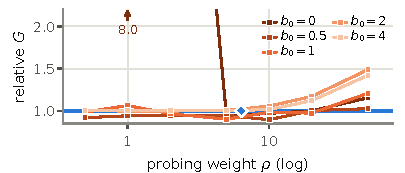
\includegraphics[width=0.32\textwidth]{fig_integrator_sensitivity}}\hfill
	\subfigure[Two-link arm, per polarity.]{\label{fig:sensitivity-arm}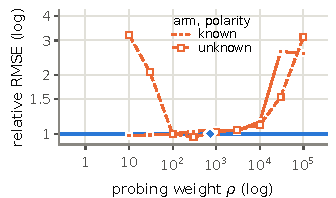
\includegraphics[width=0.32\textwidth]{fig_arm_sensitivity}}\hfill
	\subfigure[Light--dark task, per goal.]{\label{fig:lightdark-sensitivity}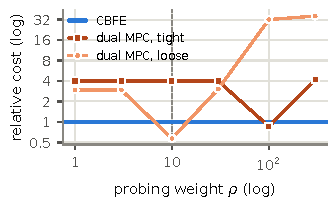
\includegraphics[width=0.32\textwidth]{fig_lightdark_sensitivity}}
	\caption{Cost of the dual MPC relative to that of CBFE against its probing weight $\rho$, on logarithmic axes. The blue line marks CBFE, which needs no tuning. The window of good weights moves by two orders of magnitude between the systems and tenfold between the goals. (a, b) RMSE, on shared axes, with the diamond at twice the median of the active multipliers of CBFE; 200 episodes per prior mean and 10 seeds per condition. (c) Goal cost, 200 episodes per goal; the dashed line marks the weight tuned on held-out seeds.}
	\label{fig:results}
\end{figure}

\subsection{ARX model: two-link arm with unknown motor polarity}\label{sec:arm}

The ARX model predicts the output from the current input and a buffer of past outputs,
\begin{equation}\label{eq:arx}
	y_k = A^\top \phi(u_k, y_{k-1}) + e_k \, , \qquad e_k \sim \cN(0, W^{-1}) \, ,
\end{equation}
so its state is the output buffer, and $\Theta = (A, W)$ collects the coefficients and the noise precision~\citep{nisslbeck2025factor}. Under a matrix normal--Wishart prior, the posterior $\mathcal{MN}(A \given M_t, \Lambda_t^{-1}, W^{-1})\, \allowbreak \mathcal{W}(W \given \Omega_t, \eta_t)$ follows in closed form~\citep{nisslbeck2025factor,gelman1995bayesian}. Its coefficient precision accumulates the features, and the leverage of a feature vector weighs it against this precision,
\begin{equation}\label{eq:leverage}
	\Lambda_k = \Lambda_{k-1} + \phi_k\phi_k^\top \, , \qquad \ell_t(\phi) = \phi^\top \Lambda_t^{-1}\phi \, .
\end{equation}
The posterior predictive is a Student-t density with covariance $(1 + \ell_t(\phi))R_t$, where $R_t$ is the posterior mean of the noise covariance.

Given $W$, the coefficients add the covariance $\ell_t W^{-1}$ to the prediction, so their information is $\tfrac{n_y}{2}\ln(1 + \ell_t(\phi))$, whereas the information about $W$ does not depend on the input. We count only the coefficient information in the constraint, because the floor measures the spread that the coefficients induce, and probing cannot raise the information about $W$. The coefficients add the covariance $\Sigma^\theta_{t+1} = \ell_t R_t$ to the prediction, so the floor is $\tfrac{n_y}{2}\ln(1 + \bar{\ell}_t) - \tfrac{1}{2}\ln|I + R_t^{-1}S_*|$, with the expected leverage $\bar{\ell}_t$ of the goal-reaching inputs. As the coefficient precision $\Lambda_t$ grows, this leverage falls, and the floor turns negative. The caution and probing terms of the first step are jointly minimised at the leverage
\begin{equation}\label{eq:leverage-opt}
	\ell^\circ = \max\big\{0,\, \gamma n_y / \tr(S_*^{-1}R_t) - 1\big\} \, ,
\end{equation}
so the multiplier that a given leverage requires scales with $\tr(S_*^{-1}R_t)/n_y$.

The arm moves in the horizontal plane with a 0.5~kg payload and torque limits of 4~N\,m, and the controllers act every 0.1~s on the joint angles. The output $y_k \in \mathbb{R}^4$ holds the joint angles and velocities, the features are constant, linear and first-harmonic Fourier terms of the torques and the previous output, and the prior comes from 600 excitation steps of a nominal simulator, tempered to the weight of 90 steps. Under unknown polarity, each seed reverses none, one or both motors, and the controllers replace their prior over the affected coefficients by a zero-mean prior. We report the RMSE of the $n = 2$ joint angles.

Fig.~\ref{fig:sensitivity-arm} shows that the window of good probing weights lies two orders of magnitude higher on the arm than on the integrator, and that CBFE finds it without tuning. Under unknown polarity, CBFE attains an RMSE of 0.525~rad, against 0.523~rad and 0.505~rad for the dual MPC tuned with a known and with an unknown polarity. The paired differences are 0.002 [$-0.022$, 0.027] and 0.020 [$-0.003$, 0.043]. Weights up to $\rho = 30$, which include the tuned weight of the integrator, apply too little torque under unknown polarity, so the arm drifts under the process noise with an RMSE of 1.09 to 1.68~rad, as for the cautious controller. With a known polarity, CBFE attains 0.503~rad against 0.501~rad for the tuned dual MPC, whereas weights from $\rho = 3\cdot 10^4$ upward more than double the RMSE. MPC-X attains 0.595~rad under unknown polarity, 0.071 [0.009, 0.138] above CBFE.

The multiplier supplies the probing weight that the unknown polarity requires and withdraws it once the model suffices for the goal. Its constraint is active on 10\% of the steps of the first round, including the first step of every seed, and never afterwards or with a known polarity. The active multipliers have a median of 363, and twice this median again lies inside the window of good weights. By~\eqref{eq:leverage-opt}, the scale $\tr(S_*^{-1}R_t)/n_y$ is 1 on the integrator and 46 on the arm, so the goal and the noise set the scale of the probing weight that tuning has to find. On one core, the planner takes a median of 9~ms per step on the arm, against a control period of 100~ms.

%\emph{Takeaway:} One CBFE configuration comes within 4\% of dual MPCs that are tuned per system and per condition, although their weights differ by two orders of magnitude between the systems.

\subsection{Hidden state: light--dark positioning}\label{sec:lightdark}

A light--dark task tests whether the goal sets the probing for a hidden state as well, where the information comes from where the agent measures~\citep{platt2010belief}. The agent regulates the state $x_k = x_{k-1} + u_k + w_k$, $w_k \sim \cN(0, 10^{-4})$, to $x_* = 0$ from $x_0 \sim \cN(0, 0.25)$, and it measures $y_k = x_k + v_k$ with $v_k \sim \cN(0, r(x_k))$. The noise variance falls smoothly from 100 for $x \leq 0$ to $10^{-3}$ for $x \geq 1.5$, so the target lies in the dark. The predicted variance does not depend on the plan, so the cautious controller has no reason to visit the light. A grid filter computes the exact posterior, whose mean $m_t$ and variance $V_t$ form the belief node.

The state information of the next output is $\mathbb{I}^x_e(u) = \tfrac{1}{2}\ln(1 + A_t/r(m_t + u))$, with the variance $A_t = V_t + q$ of the next state and the noise at its predicted mean. The goal acts on the state, so the floor is $\beta^x_t = \tfrac{1}{2}\ln(A_t/S_*)$, and the agent seeks the light until it knows its state to within the goal tolerance. We run 200 episodes of $T = 200$ steps for a tight goal, $S_* = 0.01$, and a loose one, $S_* = 0.1$, and report the goal cost per step, $(x_k - x_*)^2/(2S_*)$. Besides the cautious controller and the dual MPC, we compare belief-space planning (BSP), which propagates the variance through the most likely measurements within the plan, and the optimal controller from dynamic programming on the Gaussian belief.

Under the tight goal, CBFE attains a goal cost of 1.78 per step, against 7.12 for the cautious controller and 6.05 for BSP, whose horizon is too short to value a visit. After the first 20 steps, CBFE keeps the state within two goal standard deviations on 97\% of the steps, against 40\% for the cautious controller. The optimal controller attains 1.36, 0.42 [0.23, 0.60] below CBFE, and it returns to the light 1.2 times per episode, against 3.2 times for CBFE, which re-localises whenever the variance reaches the tolerance. Under the loose goal, CBFE attains 0.24, against 0.72 for the cautious controller and 0.13 for the optimal one.

Fig.~\ref{fig:lightdark-sensitivity} shows that no single probing weight serves both goals. The dual MPC attains 0.14 with $\rho = 10$ under the loose goal, but this weight never visits the light under the tight goal, where its cost is four times that of CBFE. Under the tight goal, only $\rho = 100$ improves on CBFE, by 0.26 [0.12, 0.37], and it parks at the light under the loose goal, at 32 times the cost of CBFE. Tuning on held-out seeds selects $\rho = 10$ for both goals, so one CBFE configuration costs less than every single weight over the two goals, whereas a weight tuned per goal costs 14\% less under the tight goal and 43\% less under the loose one.

%\emph{Takeaway:} One CBFE configuration serves goals whose tuned probing weights differ tenfold.

%%%%%%%%%%%%%%%%%%%%%%%%%%%%%%%%%%%%%%%%%%%%%%%%%%%%%%%%%%%%%%%%%%%%%%%%%%%%%%%%
\section{Discussion}\label{sec:discussion}

The information~\eqref{eq:info-constraint} has a closed form when the parameters enter the mean linearly with Gaussian noise, as in all examples, whereas nonlinear parameterisations require an approximation that perturbs both the constraint and its multiplier. The attainability of the floor relies on a parameter-induced covariance that is proportional to the noise covariance. Our planner also evaluates the floor on a grid of inputs, whose size grows exponentially with $n_u$. Constraining only the next node forces the information to come from one measurement, which costs an excursion when only distant measurements are precise, as in Section~\ref{sec:lightdark}. Constraints on later nodes would spread the probing over the plan, but they require a belief that learns within the plan, as in implicit dual control~\citep{mesbah2018stochastic}. Closed-loop stability and the consistency of the parameter estimates after the constraint switches off remain open.

%%%%%%%%%%%%%%%%%%%%%%%%%%%%%%%%%%%%%%%%%%%%%%%%%%%%%%%%%%%%%%%%%%%%%%%%%%%%%%%%
\section{Conclusion}\label{sec:conclusion}

We showed that a goal-derived information constraint turns a message passing planner on a factor graph into a dual controller without a probing weight. Variational calculus yields the posterior of the next input as the product of the control prior message and a message that weighs the expected goal log-density against the information gain. The KKT multiplier of the constraint switches probing on while the uncertainty spreads the predictions beyond the goal tolerance and off once it does not. One untuned configuration came within 2.1\% and 4\% of dual MPCs tuned for an integrator and a two-link arm, whose weights differ by two orders of magnitude, and on a light--dark task it cost less than every fixed weight over a tight and a loose goal. Future work concerns constraints on later nodes with a belief that learns within the plan.

\subsection*{Generative AI Use}

% L4DC 2027 asks authors to briefly describe any use of generative AI tools here
% (research ideation or methodology, mathematical derivations or proofs, coding or
% experimental implementation, writing or editing, literature search or synthesis),
% or to state: \textit{No generative AI tools were used in preparing this work.}
\claude{Add the generative AI statement that the L4DC template asks for.}

\acks{This work was supported by the Dutch Sectorplan Engineering.}

\bibliography{references}

%%%%%%%%%%%%%%%%%%%%%%%%%%%%%%%%%%%%%%%%%%%%%%%%%%%%%%%%%%%%%%%%%%%%%%%%%%%%%%%%
\appendix

\section{Proofs}\label{app:proofs}

\begin{proofof}{Lemma~\ref{lem:collapse}}
Under~\eqref{eq:factorization}, the factor of every conditional node cancels in its log-ratio, so the node contributes the negative entropies of its input beliefs. Equality and goal nodes contribute the negative entropy of their input as well, minus the expected goal log-density for a goal node, whereas the belief nodes of $x_t$ and $\theta$ contribute zero by Definition~\ref{def:form}. Since every edge is the input of exactly one node, these entropies cancel the edge entropies, and the control prior nodes contribute the KL divergences.
\end{proofof}

\begin{proofof}{Theorem~\ref{thm:posterior}}
The functional derivatives of~\eqref{eq:lagrangian} vanish at a stationary point. For $q(y_k)$, this gives $\lambda_{y_k} = \ln p_*$. For $q(x_k)$, it gives $\lambda_{x_k}(x_k) = \E_{p(y_k \given x_k)}[\lambda_{y_k}(y_k)] + \E_{q_{k+1}(s_{k+1} \given x_k)}[\lambda_{x_{k+1}}(x_{k+1})]$, without the second term for $k = t + K$, where $q_{k+1}$ is the belief of the next transition node. With $\nu_{d_l \to l} = \exp(\lambda_l)$, this recursion is~\eqref{eq:message}, because the equality node of $x_k$ multiplies the messages from the measurement node and the next transition node. For $q(u_k)$, it gives $\ln q(u_k) = \ln p(u_k) + \E_{q_b(s_b \given u_k)}[\lambda_{x_k}(x_k)] + \gamma_k\, \mathbb{I}_k(u_k) - 1 - \psi_k$, where $q_b$ is the belief of the transition node that consumes $u_k$, because $\mathbb{I}_{t+1}[q] = \E_{q(u_{t+1})}[\mathbb{I}_{t+1}(u_{t+1})]$ is linear in $q(u_{t+1})$ and free of the other beliefs. Unrolling the recursion along the marginalization constraints gives $\E_{q_b(s_b \given u_k)}[\lambda_{x_k}(x_k)] = \sum_{m=k}^{t+K} \E_{q(y_m \given u_k)}[\ln p_*(y_m)]$, and $\psi_k$ normalises $q(u_k)$, which gives~\eqref{eq:posterior}, the Gibbs form of control as inference~\citep{levine2018reinforcement,wainwright2008graphical}.
\end{proofof}

\begin{proofof}{Lemma~\ref{lem:multiplier}}
The multiplier weights only the information gain of the next step, so $q^\star(u;\gamma) \propto p(u)\, \nu_0(u)\, \exp\big(\gamma\, \mathbb{I}_{t+1}(u)\big)$ with a message $\nu_0 > 0$ that is free of $\gamma$. This is an exponential family with natural parameter $\gamma$ and sufficient statistic $\mathbb{I}_{t+1}$, whose log-normaliser is finite, because $\cU$ is compact and $\mathbb{I}_{t+1}$ is bounded. By the moment identities of exponential families, $h$ is the derivative of the log-normaliser, and $h'(\gamma) = \Var_{q^\star}[\mathbb{I}_{t+1}] > 0$, because $q^\star$ and $p(u)$ share their null sets. The Laplace principle gives $h(\gamma) \to \mathbb{I}^{\max}$, and complementary slackness~\eqref{eq:kkt} gives the three cases.
\end{proofof}

\end{document}
